\documentclass[twoside]{book}

% Packages required by doxygen
\usepackage{fixltx2e}
\usepackage{calc}
\usepackage{doxygen}
\usepackage[export]{adjustbox} % also loads graphicx
\usepackage{graphicx}
\usepackage[utf8]{inputenc}
\usepackage{makeidx}
\usepackage{multicol}
\usepackage{multirow}
\PassOptionsToPackage{warn}{textcomp}
\usepackage{textcomp}
\usepackage[nointegrals]{wasysym}
\usepackage[table]{xcolor}

% Font selection
\usepackage[T1]{fontenc}
\usepackage[scaled=.90]{helvet}
\usepackage{courier}
\usepackage{amssymb}
\usepackage{sectsty}
\renewcommand{\familydefault}{\sfdefault}
\allsectionsfont{%
  \fontseries{bc}\selectfont%
  \color{darkgray}%
}
\renewcommand{\DoxyLabelFont}{%
  \fontseries{bc}\selectfont%
  \color{darkgray}%
}
\newcommand{\+}{\discretionary{\mbox{\scriptsize$\hookleftarrow$}}{}{}}

% Page & text layout
\usepackage{geometry}
\geometry{%
  a4paper,%
  top=2.5cm,%
  bottom=2.5cm,%
  left=2.5cm,%
  right=2.5cm%
}
\tolerance=750
\hfuzz=15pt
\hbadness=750
\setlength{\emergencystretch}{15pt}
\setlength{\parindent}{0cm}
\setlength{\parskip}{0.2cm}
\makeatletter
\renewcommand{\paragraph}{%
  \@startsection{paragraph}{4}{0ex}{-1.0ex}{1.0ex}{%
    \normalfont\normalsize\bfseries\SS@parafont%
  }%
}
\renewcommand{\subparagraph}{%
  \@startsection{subparagraph}{5}{0ex}{-1.0ex}{1.0ex}{%
    \normalfont\normalsize\bfseries\SS@subparafont%
  }%
}
\makeatother

% Headers & footers
\usepackage{fancyhdr}
\pagestyle{fancyplain}
\fancyhead[LE]{\fancyplain{}{\bfseries\thepage}}
\fancyhead[CE]{\fancyplain{}{}}
\fancyhead[RE]{\fancyplain{}{\bfseries\leftmark}}
\fancyhead[LO]{\fancyplain{}{\bfseries\rightmark}}
\fancyhead[CO]{\fancyplain{}{}}
\fancyhead[RO]{\fancyplain{}{\bfseries\thepage}}
\fancyfoot[LE]{\fancyplain{}{}}
\fancyfoot[CE]{\fancyplain{}{}}
\fancyfoot[RE]{\fancyplain{}{\bfseries\scriptsize Generated on Sat Apr 28 2018 18\+:49\+:01 for Texture Extraction from Photographs by Doxygen }}
\fancyfoot[LO]{\fancyplain{}{\bfseries\scriptsize Generated on Sat Apr 28 2018 18\+:49\+:01 for Texture Extraction from Photographs by Doxygen }}
\fancyfoot[CO]{\fancyplain{}{}}
\fancyfoot[RO]{\fancyplain{}{}}
\renewcommand{\footrulewidth}{0.4pt}
\renewcommand{\chaptermark}[1]{%
  \markboth{#1}{}%
}
\renewcommand{\sectionmark}[1]{%
  \markright{\thesection\ #1}%
}

% Indices & bibliography
\usepackage{natbib}
\usepackage[titles]{tocloft}
\setcounter{tocdepth}{3}
\setcounter{secnumdepth}{5}
\makeindex

% Hyperlinks (required, but should be loaded last)
\usepackage{ifpdf}
\ifpdf
  \usepackage[pdftex,pagebackref=true]{hyperref}
\else
  \usepackage[ps2pdf,pagebackref=true]{hyperref}
\fi
\hypersetup{%
  colorlinks=true,%
  linkcolor=blue,%
  citecolor=blue,%
  unicode%
}

% Custom commands
\newcommand{\clearemptydoublepage}{%
  \newpage{\pagestyle{empty}\cleardoublepage}%
}


%===== C O N T E N T S =====

\begin{document}

% Titlepage & ToC
\hypersetup{pageanchor=false,
             bookmarks=true,
             bookmarksnumbered=true,
             pdfencoding=unicode
            }
\pagenumbering{roman}
\begin{titlepage}
\vspace*{7cm}
\begin{center}%
{\Large Texture Extraction from Photographs }\\
\vspace*{1cm}
{\large Generated by Doxygen 1.8.10}\\
\vspace*{0.5cm}
{\small Sat Apr 28 2018 18:49:01}\\
\end{center}
\end{titlepage}
\clearemptydoublepage
\tableofcontents
\clearemptydoublepage
\pagenumbering{arabic}
\hypersetup{pageanchor=true}

%--- Begin generated contents ---
\chapter{Hierarchical Index}
\section{Class Hierarchy}
This inheritance list is sorted roughly, but not completely, alphabetically\+:\begin{DoxyCompactList}
\item \contentsline{section}{Adjacency\+Graph}{\pageref{class_adjacency_graph}}{}
\item \contentsline{section}{Arguments}{\pageref{struct_arguments}}{}
\item \contentsline{section}{Bounding\+Box}{\pageref{struct_bounding_box}}{}
\item \contentsline{section}{Camera}{\pageref{class_camera}}{}
\item \contentsline{section}{Data\+Cost\+Extraction\+Manager}{\pageref{class_data_cost_extraction_manager}}{}
\item \contentsline{section}{Data\+Costs\+Extractor}{\pageref{class_data_costs_extractor}}{}
\item \contentsline{section}{Edge}{\pageref{class_edge}}{}
\item \contentsline{section}{Edge\+Vertex}{\pageref{struct_edge_vertex}}{}
\item \contentsline{section}{Extraction\+Worker}{\pageref{class_extraction_worker}}{}
\item \contentsline{section}{Gradient}{\pageref{class_gradient}}{}
\item \contentsline{section}{I\+N\+I\+Reader}{\pageref{class_i_n_i_reader}}{}
\item \contentsline{section}{Mesh}{\pageref{class_mesh}}{}
\item \contentsline{section}{Normal}{\pageref{struct_normal}}{}
\item \contentsline{section}{Object}{\pageref{struct_object}}{}
\item \contentsline{section}{Partition\+Node}{\pageref{struct_partition_node}}{}
\item \contentsline{section}{Patch\+Quality}{\pageref{struct_patch_quality}}{}
\item \contentsline{section}{Rasterizer}{\pageref{class_rasterizer}}{}
\item \contentsline{section}{Render\+Context}{\pageref{class_render_context}}{}
\begin{DoxyCompactList}
\item \contentsline{section}{Bitmap}{\pageref{class_bitmap}}{}
\end{DoxyCompactList}
\item \contentsline{section}{Tex\+Coord}{\pageref{struct_tex_coord}}{}
\item \contentsline{section}{Texture\+Edge}{\pageref{class_texture_edge}}{}
\item \contentsline{section}{Texture\+Extractor}{\pageref{class_texture_extractor}}{}
\item \contentsline{section}{Texture\+Gradient}{\pageref{class_texture_gradient}}{}
\item \contentsline{section}{Texture\+Patch}{\pageref{struct_texture_patch}}{}
\item \contentsline{section}{Texture\+Patch\+Dictionary}{\pageref{struct_texture_patch_dictionary}}{}
\item \contentsline{section}{Timer}{\pageref{class_timer}}{}
\item \contentsline{section}{Transformation}{\pageref{class_transformation}}{}
\item \contentsline{section}{Triangle}{\pageref{struct_triangle}}{}
\item \contentsline{section}{Vertex}{\pageref{struct_vertex}}{}
\item \contentsline{section}{View}{\pageref{class_view}}{}
\end{DoxyCompactList}

\chapter{Class Index}
\section{Class List}
Here are the classes, structs, unions and interfaces with brief descriptions\+:\begin{DoxyCompactList}
\item\contentsline{section}{\hyperlink{class_adjacency_graph}{Adjacency\+Graph} }{\pageref{class_adjacency_graph}}{}
\item\contentsline{section}{\hyperlink{struct_arguments}{Arguments} }{\pageref{struct_arguments}}{}
\item\contentsline{section}{\hyperlink{class_bitmap}{Bitmap} }{\pageref{class_bitmap}}{}
\item\contentsline{section}{\hyperlink{struct_bounding_box}{Bounding\+Box} }{\pageref{struct_bounding_box}}{}
\item\contentsline{section}{\hyperlink{class_camera}{Camera} }{\pageref{class_camera}}{}
\item\contentsline{section}{\hyperlink{class_data_cost_extraction_manager}{Data\+Cost\+Extraction\+Manager} }{\pageref{class_data_cost_extraction_manager}}{}
\item\contentsline{section}{\hyperlink{class_data_costs_extractor}{Data\+Costs\+Extractor} }{\pageref{class_data_costs_extractor}}{}
\item\contentsline{section}{\hyperlink{class_edge}{Edge} }{\pageref{class_edge}}{}
\item\contentsline{section}{\hyperlink{struct_edge_vertex}{Edge\+Vertex} }{\pageref{struct_edge_vertex}}{}
\item\contentsline{section}{\hyperlink{class_extraction_worker}{Extraction\+Worker} }{\pageref{class_extraction_worker}}{}
\item\contentsline{section}{\hyperlink{class_gradient}{Gradient} }{\pageref{class_gradient}}{}
\item\contentsline{section}{\hyperlink{class_i_n_i_reader}{I\+N\+I\+Reader} }{\pageref{class_i_n_i_reader}}{}
\item\contentsline{section}{\hyperlink{class_mesh}{Mesh} }{\pageref{class_mesh}}{}
\item\contentsline{section}{\hyperlink{struct_normal}{Normal} }{\pageref{struct_normal}}{}
\item\contentsline{section}{\hyperlink{struct_object}{Object} }{\pageref{struct_object}}{}
\item\contentsline{section}{\hyperlink{struct_partition_node}{Partition\+Node} }{\pageref{struct_partition_node}}{}
\item\contentsline{section}{\hyperlink{struct_patch_quality}{Patch\+Quality} }{\pageref{struct_patch_quality}}{}
\item\contentsline{section}{\hyperlink{class_rasterizer}{Rasterizer} }{\pageref{class_rasterizer}}{}
\item\contentsline{section}{\hyperlink{class_render_context}{Render\+Context} }{\pageref{class_render_context}}{}
\item\contentsline{section}{\hyperlink{struct_tex_coord}{Tex\+Coord} }{\pageref{struct_tex_coord}}{}
\item\contentsline{section}{\hyperlink{class_texture_edge}{Texture\+Edge} }{\pageref{class_texture_edge}}{}
\item\contentsline{section}{\hyperlink{class_texture_extractor}{Texture\+Extractor} }{\pageref{class_texture_extractor}}{}
\item\contentsline{section}{\hyperlink{class_texture_gradient}{Texture\+Gradient} }{\pageref{class_texture_gradient}}{}
\item\contentsline{section}{\hyperlink{struct_texture_patch}{Texture\+Patch} }{\pageref{struct_texture_patch}}{}
\item\contentsline{section}{\hyperlink{struct_texture_patch_dictionary}{Texture\+Patch\+Dictionary} }{\pageref{struct_texture_patch_dictionary}}{}
\item\contentsline{section}{\hyperlink{class_timer}{Timer} }{\pageref{class_timer}}{}
\item\contentsline{section}{\hyperlink{class_transformation}{Transformation} }{\pageref{class_transformation}}{}
\item\contentsline{section}{\hyperlink{struct_triangle}{Triangle} }{\pageref{struct_triangle}}{}
\item\contentsline{section}{\hyperlink{struct_vertex}{Vertex} }{\pageref{struct_vertex}}{}
\item\contentsline{section}{\hyperlink{class_view}{View} }{\pageref{class_view}}{}
\end{DoxyCompactList}

\chapter{Class Documentation}
\hypertarget{class_adjacency_graph}{}\section{Adjacency\+Graph Class Reference}
\label{class_adjacency_graph}\index{Adjacency\+Graph@{Adjacency\+Graph}}
\subsection*{Public Member Functions}
\begin{DoxyCompactItemize}
\item 
\hypertarget{class_adjacency_graph_a24a7cc8e5f62cc94872e04cfa10b70dd}{}void {\bfseries add\+Node} (uint face\+Id, const std\+::set$<$ uint $>$ \&neighbours)\label{class_adjacency_graph_a24a7cc8e5f62cc94872e04cfa10b70dd}

\end{DoxyCompactItemize}
\subsection*{Public Attributes}
\begin{DoxyCompactItemize}
\item 
\hypertarget{class_adjacency_graph_ad3e7a730db698841d4230030898f4291}{}std\+::map$<$ uint, Node $>$ {\bfseries nodes}\label{class_adjacency_graph_ad3e7a730db698841d4230030898f4291}

\end{DoxyCompactItemize}


The documentation for this class was generated from the following file\+:\begin{DoxyCompactItemize}
\item 
Texture\+Extractor\+V2/Mesh.\+hpp\end{DoxyCompactItemize}

\hypertarget{struct_arguments}{}\section{Arguments Struct Reference}
\label{struct_arguments}\index{Arguments@{Arguments}}


{\ttfamily \#include $<$Arguments.\+h$>$}



Collaboration diagram for Arguments\+:\nopagebreak
\begin{figure}[H]
\begin{center}
\leavevmode
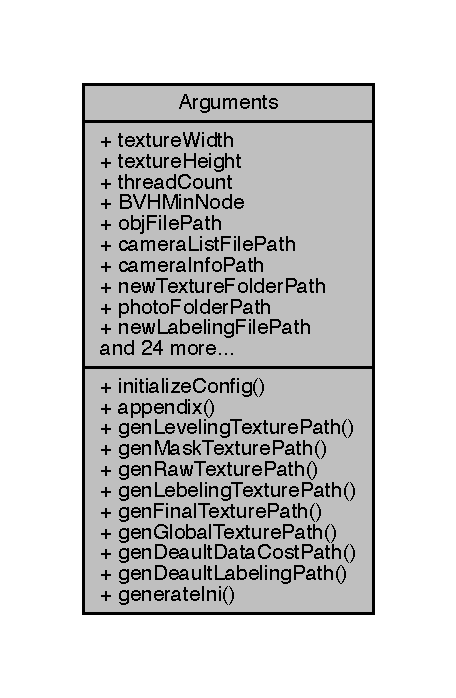
\includegraphics[width=219pt]{struct_arguments__coll__graph}
\end{center}
\end{figure}
\subsection*{Public Member Functions}
\begin{DoxyCompactItemize}
\item 
bool \hyperlink{struct_arguments_adb3df83131fa2be8783755b93c28c3de}{initialize\+Config} (std\+::string filename)
\item 
std\+::string \hyperlink{struct_arguments_a693a6a2a4334f5e34b3eb5ed6a555b28}{appendix} ()
\item 
std\+::string \hyperlink{struct_arguments_a84cff19e3bdd988ba096e1a81e747103}{gen\+Leveling\+Texture\+Path} (std\+::string obj\+Name)
\item 
std\+::string \hyperlink{struct_arguments_acc8d0c6a9477669bee3d9fe79e0b6d6c}{gen\+Mask\+Texture\+Path} (std\+::string obj\+Name)
\item 
std\+::string \hyperlink{struct_arguments_af256b45e3009486a4ea5066f8b7a080f}{gen\+Raw\+Texture\+Path} (std\+::string obj\+Name)
\item 
std\+::string \hyperlink{struct_arguments_ac2161fcafef758c6418e6d7113fedee2}{gen\+Lebeling\+Texture\+Path} (std\+::string obj\+Name)
\item 
std\+::string \hyperlink{struct_arguments_ae4c2ab8514254a581f2124d4095ffe06}{gen\+Final\+Texture\+Path} (std\+::string obj\+Name)
\item 
std\+::string \hyperlink{struct_arguments_ab6012180dadee8fff0a7271aafd96089}{gen\+Global\+Texture\+Path} (std\+::string obj\+Name)
\item 
std\+::string \hyperlink{struct_arguments_a3f54b425cb0c05cda997be2f690040a4}{gen\+Deault\+Data\+Cost\+Path} ()
\item 
std\+::string \hyperlink{struct_arguments_ad99ef1f1635874fd7dcac5b3a48dabec}{gen\+Deault\+Labeling\+Path} ()
\item 
bool \hyperlink{struct_arguments_a6db8fa82b73c39649ab151ef63085f0f}{generate\+Ini} ()
\end{DoxyCompactItemize}
\subsection*{Public Attributes}
\begin{DoxyCompactItemize}
\item 
int \hyperlink{struct_arguments_a53b1eb430f4ea67ffd9a85696a295cd0}{texture\+Width}
\item 
int \hyperlink{struct_arguments_acba64f044d4603abac85ba2cf1b50b75}{texture\+Height}
\item 
int \hyperlink{struct_arguments_a81212a8036b56467011fb90c075ec4d8}{thread\+Count}
\item 
int \hyperlink{struct_arguments_a90c008ddccf9fc27fc1e7db34b51b36e}{B\+V\+H\+Min\+Node}
\item 
std\+::string \hyperlink{struct_arguments_a5615cc24abc162c63ef3aedc135b0db4}{obj\+File\+Path}
\item 
std\+::string \hyperlink{struct_arguments_a033abba738ba0403e87f883cc203d618}{camera\+List\+File\+Path}
\item 
std\+::string \hyperlink{struct_arguments_a1efe0a7268bb4ab28a51566a13c5f36b}{camera\+Info\+Path}
\item 
std\+::string \hyperlink{struct_arguments_aacc8cf735f8d2793e4fbd81d05f22918}{new\+Texture\+Folder\+Path}
\item 
std\+::string \hyperlink{struct_arguments_a784aabe9dd9bbeb828d1ad845b72887c}{photo\+Folder\+Path}
\item 
std\+::string \hyperlink{struct_arguments_a4a043101d13a6c0540f501af85a691ce}{new\+Labeling\+File\+Path}
\item 
std\+::string \hyperlink{struct_arguments_ad753fef0a788c9868deb592ee39e0528}{labeling\+File\+Path}
\item 
std\+::string \hyperlink{struct_arguments_aaa04b2622a7712dd05c28101c149b116}{data\+Costs\+File\+Path}
\item 
std\+::string \hyperlink{struct_arguments_ae1b263850d63b7595ba4e6fd0ae525b3}{new\+Data\+Costs\+File\+Path}
\item 
std\+::string \hyperlink{struct_arguments_a5ce8b0bed244a327b762f2bb1630708b}{project\+Name}
\item 
std\+::string \hyperlink{struct_arguments_adadef95480756dd3922728cd40b8d334}{result\+Render\+Folder}
\item 
std\+::string \hyperlink{struct_arguments_af545eb82fb55577ba19adeeb5933e619}{image\+Format}
\item 
bool \hyperlink{struct_arguments_ad2a5a8782138866eacf646d57b7ea531}{get\+Labeling\+From\+File}
\item 
bool \hyperlink{struct_arguments_ac81dde9796306362b5c06f2d62a901ea}{write\+Labeling\+To\+File}
\item 
bool \hyperlink{struct_arguments_a36e514162f0dca494ae8b558016fba23}{get\+Data\+Costs\+From\+File}
\item 
bool \hyperlink{struct_arguments_a3f797aec500d79580f523addf2a62786}{write\+Data\+Costs\+To\+File}
\item 
bool \hyperlink{struct_arguments_a35c85467eaefb45dd9c5573c5697d0be}{do\+Gloabal\+Adjustment}
\item 
bool \hyperlink{struct_arguments_a37157aeefb4bab06270e0787c0bac2cb}{do\+Seam\+Leveling}
\item 
bool \hyperlink{struct_arguments_aa8074aacbc6ee3f99effd5b7613905e5}{do\+Texture\+Extension}
\item 
bool \hyperlink{struct_arguments_aba3898efc576d5bd85f4f89e7b0b79a6}{do\+Color\+Consistency}
\item 
float \hyperlink{struct_arguments_a427521a6262f69340de5f09fdb3292d0}{color\+Consistency\+Threshold}
\item 
bool \hyperlink{struct_arguments_a50abe906778cd4d167400327224437aa}{gen\+Lebeling\+Texture}
\item 
bool \hyperlink{struct_arguments_a3cb31e33468d5ac33e53a155da84b3d2}{gen\+Leveling\+Texture}
\item 
bool \hyperlink{struct_arguments_acada25027fb72d5a7d8440b62653af2f}{gen\+Mask\+Texture}
\item 
bool \hyperlink{struct_arguments_ac401fe9a04307aa31bda75d4424ceed3}{gen\+Global\+Texture}
\item 
bool \hyperlink{struct_arguments_afe5ecd92c78f3f5a6b751139ec50ee6f}{gen\+Raw\+Texture}
\item 
bool \hyperlink{struct_arguments_ab0a6f926571b9ebd895f84af4214880b}{strict\+Oclusion\+Check}
\item 
bool \hyperlink{struct_arguments_a5438dd5f419d88e72ba7dad3e7343229}{add\+Project\+Name\+To\+Files}
\item 
bool \hyperlink{struct_arguments_a425be50cc8828826b939677321ae98dc}{\+\_\+just\+Render}
\item 
bool \hyperlink{struct_arguments_ada75eb1bead23d95007b7a757050015e}{\+\_\+render\+In\+The\+End}
\end{DoxyCompactItemize}


\subsection{Detailed Description}
Structure that manages all the argument checking and reading. 

\subsection{Member Function Documentation}
\hypertarget{struct_arguments_a693a6a2a4334f5e34b3eb5ed6a555b28}{}\index{Arguments@{Arguments}!appendix@{appendix}}
\index{appendix@{appendix}!Arguments@{Arguments}}
\subsubsection[{appendix()}]{\setlength{\rightskip}{0pt plus 5cm}std\+::string Arguments\+::appendix (
\begin{DoxyParamCaption}
{}
\end{DoxyParamCaption}
)\hspace{0.3cm}{\ttfamily [inline]}}\label{struct_arguments_a693a6a2a4334f5e34b3eb5ed6a555b28}
Return file appendix to add to the begining of file \hypertarget{struct_arguments_a3f54b425cb0c05cda997be2f690040a4}{}\index{Arguments@{Arguments}!gen\+Deault\+Data\+Cost\+Path@{gen\+Deault\+Data\+Cost\+Path}}
\index{gen\+Deault\+Data\+Cost\+Path@{gen\+Deault\+Data\+Cost\+Path}!Arguments@{Arguments}}
\subsubsection[{gen\+Deault\+Data\+Cost\+Path()}]{\setlength{\rightskip}{0pt plus 5cm}std\+::string Arguments\+::gen\+Deault\+Data\+Cost\+Path (
\begin{DoxyParamCaption}
{}
\end{DoxyParamCaption}
)\hspace{0.3cm}{\ttfamily [inline]}}\label{struct_arguments_a3f54b425cb0c05cda997be2f690040a4}
Returns a default path to data cost file \begin{DoxyReturn}{Returns}
path and name for a data cost file 
\end{DoxyReturn}
\hypertarget{struct_arguments_ad99ef1f1635874fd7dcac5b3a48dabec}{}\index{Arguments@{Arguments}!gen\+Deault\+Labeling\+Path@{gen\+Deault\+Labeling\+Path}}
\index{gen\+Deault\+Labeling\+Path@{gen\+Deault\+Labeling\+Path}!Arguments@{Arguments}}
\subsubsection[{gen\+Deault\+Labeling\+Path()}]{\setlength{\rightskip}{0pt plus 5cm}std\+::string Arguments\+::gen\+Deault\+Labeling\+Path (
\begin{DoxyParamCaption}
{}
\end{DoxyParamCaption}
)\hspace{0.3cm}{\ttfamily [inline]}}\label{struct_arguments_ad99ef1f1635874fd7dcac5b3a48dabec}
Returns a default path to labeling file \begin{DoxyReturn}{Returns}
path and name for a labeling file 
\end{DoxyReturn}
\hypertarget{struct_arguments_a6db8fa82b73c39649ab151ef63085f0f}{}\index{Arguments@{Arguments}!generate\+Ini@{generate\+Ini}}
\index{generate\+Ini@{generate\+Ini}!Arguments@{Arguments}}
\subsubsection[{generate\+Ini()}]{\setlength{\rightskip}{0pt plus 5cm}bool Arguments\+::generate\+Ini (
\begin{DoxyParamCaption}
{}
\end{DoxyParamCaption}
)\hspace{0.3cm}{\ttfamily [inline]}}\label{struct_arguments_a6db8fa82b73c39649ab151ef63085f0f}
Generates an example ini file \begin{DoxyReturn}{Returns}
true if generation successful 
\end{DoxyReturn}
\hypertarget{struct_arguments_ae4c2ab8514254a581f2124d4095ffe06}{}\index{Arguments@{Arguments}!gen\+Final\+Texture\+Path@{gen\+Final\+Texture\+Path}}
\index{gen\+Final\+Texture\+Path@{gen\+Final\+Texture\+Path}!Arguments@{Arguments}}
\subsubsection[{gen\+Final\+Texture\+Path(std\+::string obj\+Name)}]{\setlength{\rightskip}{0pt plus 5cm}std\+::string Arguments\+::gen\+Final\+Texture\+Path (
\begin{DoxyParamCaption}
\item[{std\+::string}]{obj\+Name}
\end{DoxyParamCaption}
)\hspace{0.3cm}{\ttfamily [inline]}}\label{struct_arguments_ae4c2ab8514254a581f2124d4095ffe06}
Returns path to final texture for an object 
\begin{DoxyParams}{Parameters}
{\em obj\+Name} & object name. \\
\hline
\end{DoxyParams}
\begin{DoxyReturn}{Returns}
path and name for a new final texture 
\end{DoxyReturn}
\hypertarget{struct_arguments_ab6012180dadee8fff0a7271aafd96089}{}\index{Arguments@{Arguments}!gen\+Global\+Texture\+Path@{gen\+Global\+Texture\+Path}}
\index{gen\+Global\+Texture\+Path@{gen\+Global\+Texture\+Path}!Arguments@{Arguments}}
\subsubsection[{gen\+Global\+Texture\+Path(std\+::string obj\+Name)}]{\setlength{\rightskip}{0pt plus 5cm}std\+::string Arguments\+::gen\+Global\+Texture\+Path (
\begin{DoxyParamCaption}
\item[{std\+::string}]{obj\+Name}
\end{DoxyParamCaption}
)\hspace{0.3cm}{\ttfamily [inline]}}\label{struct_arguments_ab6012180dadee8fff0a7271aafd96089}
Returns path to global texture for an object 
\begin{DoxyParams}{Parameters}
{\em obj\+Name} & object name. \\
\hline
\end{DoxyParams}
\begin{DoxyReturn}{Returns}
path and name for a new global texture 
\end{DoxyReturn}
\hypertarget{struct_arguments_ac2161fcafef758c6418e6d7113fedee2}{}\index{Arguments@{Arguments}!gen\+Lebeling\+Texture\+Path@{gen\+Lebeling\+Texture\+Path}}
\index{gen\+Lebeling\+Texture\+Path@{gen\+Lebeling\+Texture\+Path}!Arguments@{Arguments}}
\subsubsection[{gen\+Lebeling\+Texture\+Path(std\+::string obj\+Name)}]{\setlength{\rightskip}{0pt plus 5cm}std\+::string Arguments\+::gen\+Lebeling\+Texture\+Path (
\begin{DoxyParamCaption}
\item[{std\+::string}]{obj\+Name}
\end{DoxyParamCaption}
)\hspace{0.3cm}{\ttfamily [inline]}}\label{struct_arguments_ac2161fcafef758c6418e6d7113fedee2}
Returns path to lebeling texture for an object 
\begin{DoxyParams}{Parameters}
{\em obj\+Name} & object name. \\
\hline
\end{DoxyParams}
\begin{DoxyReturn}{Returns}
path and name for a new lebeling texture 
\end{DoxyReturn}
\hypertarget{struct_arguments_a84cff19e3bdd988ba096e1a81e747103}{}\index{Arguments@{Arguments}!gen\+Leveling\+Texture\+Path@{gen\+Leveling\+Texture\+Path}}
\index{gen\+Leveling\+Texture\+Path@{gen\+Leveling\+Texture\+Path}!Arguments@{Arguments}}
\subsubsection[{gen\+Leveling\+Texture\+Path(std\+::string obj\+Name)}]{\setlength{\rightskip}{0pt plus 5cm}std\+::string Arguments\+::gen\+Leveling\+Texture\+Path (
\begin{DoxyParamCaption}
\item[{std\+::string}]{obj\+Name}
\end{DoxyParamCaption}
)\hspace{0.3cm}{\ttfamily [inline]}}\label{struct_arguments_a84cff19e3bdd988ba096e1a81e747103}
Returns path to leveling texture for an object 
\begin{DoxyParams}{Parameters}
{\em obj\+Name} & object name. \\
\hline
\end{DoxyParams}
\begin{DoxyReturn}{Returns}
path and name for a new leveling texture 
\end{DoxyReturn}
\hypertarget{struct_arguments_acc8d0c6a9477669bee3d9fe79e0b6d6c}{}\index{Arguments@{Arguments}!gen\+Mask\+Texture\+Path@{gen\+Mask\+Texture\+Path}}
\index{gen\+Mask\+Texture\+Path@{gen\+Mask\+Texture\+Path}!Arguments@{Arguments}}
\subsubsection[{gen\+Mask\+Texture\+Path(std\+::string obj\+Name)}]{\setlength{\rightskip}{0pt plus 5cm}std\+::string Arguments\+::gen\+Mask\+Texture\+Path (
\begin{DoxyParamCaption}
\item[{std\+::string}]{obj\+Name}
\end{DoxyParamCaption}
)\hspace{0.3cm}{\ttfamily [inline]}}\label{struct_arguments_acc8d0c6a9477669bee3d9fe79e0b6d6c}
Returns path to mask texture for an object 
\begin{DoxyParams}{Parameters}
{\em obj\+Name} & object name. \\
\hline
\end{DoxyParams}
\begin{DoxyReturn}{Returns}
path and name for a new mask texture 
\end{DoxyReturn}
\hypertarget{struct_arguments_af256b45e3009486a4ea5066f8b7a080f}{}\index{Arguments@{Arguments}!gen\+Raw\+Texture\+Path@{gen\+Raw\+Texture\+Path}}
\index{gen\+Raw\+Texture\+Path@{gen\+Raw\+Texture\+Path}!Arguments@{Arguments}}
\subsubsection[{gen\+Raw\+Texture\+Path(std\+::string obj\+Name)}]{\setlength{\rightskip}{0pt plus 5cm}std\+::string Arguments\+::gen\+Raw\+Texture\+Path (
\begin{DoxyParamCaption}
\item[{std\+::string}]{obj\+Name}
\end{DoxyParamCaption}
)\hspace{0.3cm}{\ttfamily [inline]}}\label{struct_arguments_af256b45e3009486a4ea5066f8b7a080f}
Returns path to raw texture for an object 
\begin{DoxyParams}{Parameters}
{\em obj\+Name} & object name. \\
\hline
\end{DoxyParams}
\begin{DoxyReturn}{Returns}
path and name for a new raw texture 
\end{DoxyReturn}
\hypertarget{struct_arguments_adb3df83131fa2be8783755b93c28c3de}{}\index{Arguments@{Arguments}!initialize\+Config@{initialize\+Config}}
\index{initialize\+Config@{initialize\+Config}!Arguments@{Arguments}}
\subsubsection[{initialize\+Config(std\+::string filename)}]{\setlength{\rightskip}{0pt plus 5cm}bool Arguments\+::initialize\+Config (
\begin{DoxyParamCaption}
\item[{std\+::string}]{filename}
\end{DoxyParamCaption}
)\hspace{0.3cm}{\ttfamily [inline]}}\label{struct_arguments_adb3df83131fa2be8783755b93c28c3de}
Read and verify the consiguration file§ 
\begin{DoxyParams}{Parameters}
{\em filename} & Pacth to the ini config \\
\hline
\end{DoxyParams}
\begin{DoxyReturn}{Returns}
true if all went well. 
\end{DoxyReturn}


\subsection{Member Data Documentation}
\hypertarget{struct_arguments_a425be50cc8828826b939677321ae98dc}{}\index{Arguments@{Arguments}!\+\_\+just\+Render@{\+\_\+just\+Render}}
\index{\+\_\+just\+Render@{\+\_\+just\+Render}!Arguments@{Arguments}}
\subsubsection[{\+\_\+just\+Render}]{\setlength{\rightskip}{0pt plus 5cm}bool Arguments\+::\+\_\+just\+Render}\label{struct_arguments_a425be50cc8828826b939677321ae98dc}
D\+E\+B\+U\+G\+: ask program to only render test renders \hypertarget{struct_arguments_ada75eb1bead23d95007b7a757050015e}{}\index{Arguments@{Arguments}!\+\_\+render\+In\+The\+End@{\+\_\+render\+In\+The\+End}}
\index{\+\_\+render\+In\+The\+End@{\+\_\+render\+In\+The\+End}!Arguments@{Arguments}}
\subsubsection[{\+\_\+render\+In\+The\+End}]{\setlength{\rightskip}{0pt plus 5cm}bool Arguments\+::\+\_\+render\+In\+The\+End}\label{struct_arguments_ada75eb1bead23d95007b7a757050015e}
D\+E\+B\+U\+G\+: ask program to render test renders after program execution \hypertarget{struct_arguments_a5438dd5f419d88e72ba7dad3e7343229}{}\index{Arguments@{Arguments}!add\+Project\+Name\+To\+Files@{add\+Project\+Name\+To\+Files}}
\index{add\+Project\+Name\+To\+Files@{add\+Project\+Name\+To\+Files}!Arguments@{Arguments}}
\subsubsection[{add\+Project\+Name\+To\+Files}]{\setlength{\rightskip}{0pt plus 5cm}bool Arguments\+::add\+Project\+Name\+To\+Files}\label{struct_arguments_a5438dd5f419d88e72ba7dad3e7343229}
flag that defines if tool should add project\+Name to files \hypertarget{struct_arguments_a90c008ddccf9fc27fc1e7db34b51b36e}{}\index{Arguments@{Arguments}!B\+V\+H\+Min\+Node@{B\+V\+H\+Min\+Node}}
\index{B\+V\+H\+Min\+Node@{B\+V\+H\+Min\+Node}!Arguments@{Arguments}}
\subsubsection[{B\+V\+H\+Min\+Node}]{\setlength{\rightskip}{0pt plus 5cm}int Arguments\+::\+B\+V\+H\+Min\+Node}\label{struct_arguments_a90c008ddccf9fc27fc1e7db34b51b36e}
size of the minimal node. Used for constructing Bounding Volume Hierrachy \hypertarget{struct_arguments_a1efe0a7268bb4ab28a51566a13c5f36b}{}\index{Arguments@{Arguments}!camera\+Info\+Path@{camera\+Info\+Path}}
\index{camera\+Info\+Path@{camera\+Info\+Path}!Arguments@{Arguments}}
\subsubsection[{camera\+Info\+Path}]{\setlength{\rightskip}{0pt plus 5cm}std\+::string Arguments\+::camera\+Info\+Path}\label{struct_arguments_a1efe0a7268bb4ab28a51566a13c5f36b}
path to blundler file \textquotesingle{}bundle.\+rd.\+out\textquotesingle{} \hypertarget{struct_arguments_a033abba738ba0403e87f883cc203d618}{}\index{Arguments@{Arguments}!camera\+List\+File\+Path@{camera\+List\+File\+Path}}
\index{camera\+List\+File\+Path@{camera\+List\+File\+Path}!Arguments@{Arguments}}
\subsubsection[{camera\+List\+File\+Path}]{\setlength{\rightskip}{0pt plus 5cm}std\+::string Arguments\+::camera\+List\+File\+Path}\label{struct_arguments_a033abba738ba0403e87f883cc203d618}
path to list that contrains paths to photos \hypertarget{struct_arguments_a427521a6262f69340de5f09fdb3292d0}{}\index{Arguments@{Arguments}!color\+Consistency\+Threshold@{color\+Consistency\+Threshold}}
\index{color\+Consistency\+Threshold@{color\+Consistency\+Threshold}!Arguments@{Arguments}}
\subsubsection[{color\+Consistency\+Threshold}]{\setlength{\rightskip}{0pt plus 5cm}float Arguments\+::color\+Consistency\+Threshold}\label{struct_arguments_a427521a6262f69340de5f09fdb3292d0}
delta derivation from the mean limit. Makes color consistency check stricter \hypertarget{struct_arguments_aaa04b2622a7712dd05c28101c149b116}{}\index{Arguments@{Arguments}!data\+Costs\+File\+Path@{data\+Costs\+File\+Path}}
\index{data\+Costs\+File\+Path@{data\+Costs\+File\+Path}!Arguments@{Arguments}}
\subsubsection[{data\+Costs\+File\+Path}]{\setlength{\rightskip}{0pt plus 5cm}std\+::string Arguments\+::data\+Costs\+File\+Path}\label{struct_arguments_aaa04b2622a7712dd05c28101c149b116}
path to the data cost file for reading \hypertarget{struct_arguments_aba3898efc576d5bd85f4f89e7b0b79a6}{}\index{Arguments@{Arguments}!do\+Color\+Consistency@{do\+Color\+Consistency}}
\index{do\+Color\+Consistency@{do\+Color\+Consistency}!Arguments@{Arguments}}
\subsubsection[{do\+Color\+Consistency}]{\setlength{\rightskip}{0pt plus 5cm}bool Arguments\+::do\+Color\+Consistency}\label{struct_arguments_aba3898efc576d5bd85f4f89e7b0b79a6}
flag that defines if tool will perform color consistency check \hypertarget{struct_arguments_a35c85467eaefb45dd9c5573c5697d0be}{}\index{Arguments@{Arguments}!do\+Gloabal\+Adjustment@{do\+Gloabal\+Adjustment}}
\index{do\+Gloabal\+Adjustment@{do\+Gloabal\+Adjustment}!Arguments@{Arguments}}
\subsubsection[{do\+Gloabal\+Adjustment}]{\setlength{\rightskip}{0pt plus 5cm}bool Arguments\+::do\+Gloabal\+Adjustment}\label{struct_arguments_a35c85467eaefb45dd9c5573c5697d0be}
flag that defines if tool will perform global adjestement step \hypertarget{struct_arguments_a37157aeefb4bab06270e0787c0bac2cb}{}\index{Arguments@{Arguments}!do\+Seam\+Leveling@{do\+Seam\+Leveling}}
\index{do\+Seam\+Leveling@{do\+Seam\+Leveling}!Arguments@{Arguments}}
\subsubsection[{do\+Seam\+Leveling}]{\setlength{\rightskip}{0pt plus 5cm}bool Arguments\+::do\+Seam\+Leveling}\label{struct_arguments_a37157aeefb4bab06270e0787c0bac2cb}
flag that defines if tool will perform seam leveling step \hypertarget{struct_arguments_aa8074aacbc6ee3f99effd5b7613905e5}{}\index{Arguments@{Arguments}!do\+Texture\+Extension@{do\+Texture\+Extension}}
\index{do\+Texture\+Extension@{do\+Texture\+Extension}!Arguments@{Arguments}}
\subsubsection[{do\+Texture\+Extension}]{\setlength{\rightskip}{0pt plus 5cm}bool Arguments\+::do\+Texture\+Extension}\label{struct_arguments_aa8074aacbc6ee3f99effd5b7613905e5}
flag that defines if tool will perform texture extension step \hypertarget{struct_arguments_ac401fe9a04307aa31bda75d4424ceed3}{}\index{Arguments@{Arguments}!gen\+Global\+Texture@{gen\+Global\+Texture}}
\index{gen\+Global\+Texture@{gen\+Global\+Texture}!Arguments@{Arguments}}
\subsubsection[{gen\+Global\+Texture}]{\setlength{\rightskip}{0pt plus 5cm}bool Arguments\+::gen\+Global\+Texture}\label{struct_arguments_ac401fe9a04307aa31bda75d4424ceed3}
D\+E\+B\+U\+G\+: should the \textquotesingle{}global\textquotesingle{} texture be generated on its on \hypertarget{struct_arguments_a50abe906778cd4d167400327224437aa}{}\index{Arguments@{Arguments}!gen\+Lebeling\+Texture@{gen\+Lebeling\+Texture}}
\index{gen\+Lebeling\+Texture@{gen\+Lebeling\+Texture}!Arguments@{Arguments}}
\subsubsection[{gen\+Lebeling\+Texture}]{\setlength{\rightskip}{0pt plus 5cm}bool Arguments\+::gen\+Lebeling\+Texture}\label{struct_arguments_a50abe906778cd4d167400327224437aa}
D\+E\+B\+U\+G\+: should the \textquotesingle{}labeling\textquotesingle{} texture be generated on its on \hypertarget{struct_arguments_a3cb31e33468d5ac33e53a155da84b3d2}{}\index{Arguments@{Arguments}!gen\+Leveling\+Texture@{gen\+Leveling\+Texture}}
\index{gen\+Leveling\+Texture@{gen\+Leveling\+Texture}!Arguments@{Arguments}}
\subsubsection[{gen\+Leveling\+Texture}]{\setlength{\rightskip}{0pt plus 5cm}bool Arguments\+::gen\+Leveling\+Texture}\label{struct_arguments_a3cb31e33468d5ac33e53a155da84b3d2}
D\+E\+B\+U\+G\+: should the \textquotesingle{}leveling\textquotesingle{} texture be generated on its on \hypertarget{struct_arguments_acada25027fb72d5a7d8440b62653af2f}{}\index{Arguments@{Arguments}!gen\+Mask\+Texture@{gen\+Mask\+Texture}}
\index{gen\+Mask\+Texture@{gen\+Mask\+Texture}!Arguments@{Arguments}}
\subsubsection[{gen\+Mask\+Texture}]{\setlength{\rightskip}{0pt plus 5cm}bool Arguments\+::gen\+Mask\+Texture}\label{struct_arguments_acada25027fb72d5a7d8440b62653af2f}
D\+E\+B\+U\+G\+: should the \textquotesingle{}mask\textquotesingle{} texture be generated on its on \hypertarget{struct_arguments_afe5ecd92c78f3f5a6b751139ec50ee6f}{}\index{Arguments@{Arguments}!gen\+Raw\+Texture@{gen\+Raw\+Texture}}
\index{gen\+Raw\+Texture@{gen\+Raw\+Texture}!Arguments@{Arguments}}
\subsubsection[{gen\+Raw\+Texture}]{\setlength{\rightskip}{0pt plus 5cm}bool Arguments\+::gen\+Raw\+Texture}\label{struct_arguments_afe5ecd92c78f3f5a6b751139ec50ee6f}
D\+E\+B\+U\+G\+: should the \textquotesingle{}raw\textquotesingle{} texture be generated on its on \hypertarget{struct_arguments_a36e514162f0dca494ae8b558016fba23}{}\index{Arguments@{Arguments}!get\+Data\+Costs\+From\+File@{get\+Data\+Costs\+From\+File}}
\index{get\+Data\+Costs\+From\+File@{get\+Data\+Costs\+From\+File}!Arguments@{Arguments}}
\subsubsection[{get\+Data\+Costs\+From\+File}]{\setlength{\rightskip}{0pt plus 5cm}bool Arguments\+::get\+Data\+Costs\+From\+File}\label{struct_arguments_a36e514162f0dca494ae8b558016fba23}
flag that defines if tool will attempt to get data costs from the file \hypertarget{struct_arguments_ad2a5a8782138866eacf646d57b7ea531}{}\index{Arguments@{Arguments}!get\+Labeling\+From\+File@{get\+Labeling\+From\+File}}
\index{get\+Labeling\+From\+File@{get\+Labeling\+From\+File}!Arguments@{Arguments}}
\subsubsection[{get\+Labeling\+From\+File}]{\setlength{\rightskip}{0pt plus 5cm}bool Arguments\+::get\+Labeling\+From\+File}\label{struct_arguments_ad2a5a8782138866eacf646d57b7ea531}
flag that defines if tool will attempt to get labeling from the file \hypertarget{struct_arguments_af545eb82fb55577ba19adeeb5933e619}{}\index{Arguments@{Arguments}!image\+Format@{image\+Format}}
\index{image\+Format@{image\+Format}!Arguments@{Arguments}}
\subsubsection[{image\+Format}]{\setlength{\rightskip}{0pt plus 5cm}std\+::string Arguments\+::image\+Format}\label{struct_arguments_af545eb82fb55577ba19adeeb5933e619}
string containing the output image format \hypertarget{struct_arguments_ad753fef0a788c9868deb592ee39e0528}{}\index{Arguments@{Arguments}!labeling\+File\+Path@{labeling\+File\+Path}}
\index{labeling\+File\+Path@{labeling\+File\+Path}!Arguments@{Arguments}}
\subsubsection[{labeling\+File\+Path}]{\setlength{\rightskip}{0pt plus 5cm}std\+::string Arguments\+::labeling\+File\+Path}\label{struct_arguments_ad753fef0a788c9868deb592ee39e0528}
path to the labeling file for reading \hypertarget{struct_arguments_ae1b263850d63b7595ba4e6fd0ae525b3}{}\index{Arguments@{Arguments}!new\+Data\+Costs\+File\+Path@{new\+Data\+Costs\+File\+Path}}
\index{new\+Data\+Costs\+File\+Path@{new\+Data\+Costs\+File\+Path}!Arguments@{Arguments}}
\subsubsection[{new\+Data\+Costs\+File\+Path}]{\setlength{\rightskip}{0pt plus 5cm}std\+::string Arguments\+::new\+Data\+Costs\+File\+Path}\label{struct_arguments_ae1b263850d63b7595ba4e6fd0ae525b3}
path and name of ned data cost file \hypertarget{struct_arguments_a4a043101d13a6c0540f501af85a691ce}{}\index{Arguments@{Arguments}!new\+Labeling\+File\+Path@{new\+Labeling\+File\+Path}}
\index{new\+Labeling\+File\+Path@{new\+Labeling\+File\+Path}!Arguments@{Arguments}}
\subsubsection[{new\+Labeling\+File\+Path}]{\setlength{\rightskip}{0pt plus 5cm}std\+::string Arguments\+::new\+Labeling\+File\+Path}\label{struct_arguments_a4a043101d13a6c0540f501af85a691ce}
path and name of the output labeling \hypertarget{struct_arguments_aacc8cf735f8d2793e4fbd81d05f22918}{}\index{Arguments@{Arguments}!new\+Texture\+Folder\+Path@{new\+Texture\+Folder\+Path}}
\index{new\+Texture\+Folder\+Path@{new\+Texture\+Folder\+Path}!Arguments@{Arguments}}
\subsubsection[{new\+Texture\+Folder\+Path}]{\setlength{\rightskip}{0pt plus 5cm}std\+::string Arguments\+::new\+Texture\+Folder\+Path}\label{struct_arguments_aacc8cf735f8d2793e4fbd81d05f22918}
path to the output directory \hypertarget{struct_arguments_a5615cc24abc162c63ef3aedc135b0db4}{}\index{Arguments@{Arguments}!obj\+File\+Path@{obj\+File\+Path}}
\index{obj\+File\+Path@{obj\+File\+Path}!Arguments@{Arguments}}
\subsubsection[{obj\+File\+Path}]{\setlength{\rightskip}{0pt plus 5cm}std\+::string Arguments\+::obj\+File\+Path}\label{struct_arguments_a5615cc24abc162c63ef3aedc135b0db4}
path to an obj file \hypertarget{struct_arguments_a784aabe9dd9bbeb828d1ad845b72887c}{}\index{Arguments@{Arguments}!photo\+Folder\+Path@{photo\+Folder\+Path}}
\index{photo\+Folder\+Path@{photo\+Folder\+Path}!Arguments@{Arguments}}
\subsubsection[{photo\+Folder\+Path}]{\setlength{\rightskip}{0pt plus 5cm}std\+::string Arguments\+::photo\+Folder\+Path}\label{struct_arguments_a784aabe9dd9bbeb828d1ad845b72887c}
folder that gets added to the beginng of the path for the photograph paths in the camera\+List\+File\+Path \hypertarget{struct_arguments_a5ce8b0bed244a327b762f2bb1630708b}{}\index{Arguments@{Arguments}!project\+Name@{project\+Name}}
\index{project\+Name@{project\+Name}!Arguments@{Arguments}}
\subsubsection[{project\+Name}]{\setlength{\rightskip}{0pt plus 5cm}std\+::string Arguments\+::project\+Name}\label{struct_arguments_a5ce8b0bed244a327b762f2bb1630708b}
project name for a given dataset \hypertarget{struct_arguments_adadef95480756dd3922728cd40b8d334}{}\index{Arguments@{Arguments}!result\+Render\+Folder@{result\+Render\+Folder}}
\index{result\+Render\+Folder@{result\+Render\+Folder}!Arguments@{Arguments}}
\subsubsection[{result\+Render\+Folder}]{\setlength{\rightskip}{0pt plus 5cm}std\+::string Arguments\+::result\+Render\+Folder}\label{struct_arguments_adadef95480756dd3922728cd40b8d334}
folder to outtput debug denders \hypertarget{struct_arguments_ab0a6f926571b9ebd895f84af4214880b}{}\index{Arguments@{Arguments}!strict\+Oclusion\+Check@{strict\+Oclusion\+Check}}
\index{strict\+Oclusion\+Check@{strict\+Oclusion\+Check}!Arguments@{Arguments}}
\subsubsection[{strict\+Oclusion\+Check}]{\setlength{\rightskip}{0pt plus 5cm}bool Arguments\+::strict\+Oclusion\+Check}\label{struct_arguments_ab0a6f926571b9ebd895f84af4214880b}
flag that defines if tool will do a strict oclusion check. If T\+R\+U\+E even if a fragment is ocluded by only one pixel its triangle-\/view pair get discarded. if F\+A\+L\+S\+E only the view-\/triangle pairs where triangle is fully invisible get discarded \hypertarget{struct_arguments_acba64f044d4603abac85ba2cf1b50b75}{}\index{Arguments@{Arguments}!texture\+Height@{texture\+Height}}
\index{texture\+Height@{texture\+Height}!Arguments@{Arguments}}
\subsubsection[{texture\+Height}]{\setlength{\rightskip}{0pt plus 5cm}int Arguments\+::texture\+Height}\label{struct_arguments_acba64f044d4603abac85ba2cf1b50b75}
output file texture height \hypertarget{struct_arguments_a53b1eb430f4ea67ffd9a85696a295cd0}{}\index{Arguments@{Arguments}!texture\+Width@{texture\+Width}}
\index{texture\+Width@{texture\+Width}!Arguments@{Arguments}}
\subsubsection[{texture\+Width}]{\setlength{\rightskip}{0pt plus 5cm}int Arguments\+::texture\+Width}\label{struct_arguments_a53b1eb430f4ea67ffd9a85696a295cd0}
output file texture width \hypertarget{struct_arguments_a81212a8036b56467011fb90c075ec4d8}{}\index{Arguments@{Arguments}!thread\+Count@{thread\+Count}}
\index{thread\+Count@{thread\+Count}!Arguments@{Arguments}}
\subsubsection[{thread\+Count}]{\setlength{\rightskip}{0pt plus 5cm}int Arguments\+::thread\+Count}\label{struct_arguments_a81212a8036b56467011fb90c075ec4d8}
number of working threads used during data cost extraction \hypertarget{struct_arguments_a3f797aec500d79580f523addf2a62786}{}\index{Arguments@{Arguments}!write\+Data\+Costs\+To\+File@{write\+Data\+Costs\+To\+File}}
\index{write\+Data\+Costs\+To\+File@{write\+Data\+Costs\+To\+File}!Arguments@{Arguments}}
\subsubsection[{write\+Data\+Costs\+To\+File}]{\setlength{\rightskip}{0pt plus 5cm}bool Arguments\+::write\+Data\+Costs\+To\+File}\label{struct_arguments_a3f797aec500d79580f523addf2a62786}
flag that defines if tool will attempt to write data costs into the file \hypertarget{struct_arguments_ac81dde9796306362b5c06f2d62a901ea}{}\index{Arguments@{Arguments}!write\+Labeling\+To\+File@{write\+Labeling\+To\+File}}
\index{write\+Labeling\+To\+File@{write\+Labeling\+To\+File}!Arguments@{Arguments}}
\subsubsection[{write\+Labeling\+To\+File}]{\setlength{\rightskip}{0pt plus 5cm}bool Arguments\+::write\+Labeling\+To\+File}\label{struct_arguments_ac81dde9796306362b5c06f2d62a901ea}
flag that defines if tool will attempt to write labeling into the file 

The documentation for this struct was generated from the following file\+:\begin{DoxyCompactItemize}
\item 
Texture\+Extractor\+V2/\hyperlink{_arguments_8h}{Arguments.\+h}\end{DoxyCompactItemize}

\hypertarget{class_bitmap}{}\section{Bitmap Class Reference}
\label{class_bitmap}\index{Bitmap@{Bitmap}}
Inheritance diagram for Bitmap\+:\begin{figure}[H]
\begin{center}
\leavevmode
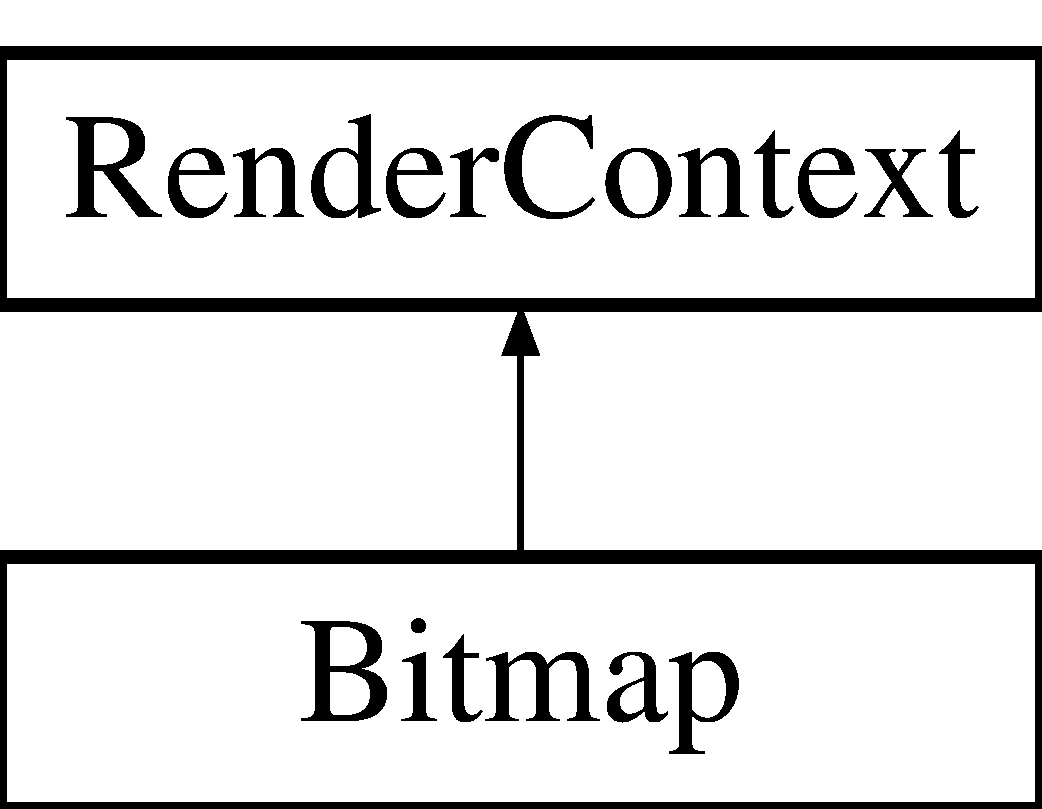
\includegraphics[height=2.000000cm]{class_bitmap}
\end{center}
\end{figure}
\subsection*{Public Member Functions}
\begin{DoxyCompactItemize}
\item 
\hypertarget{class_bitmap_a7a1a9969ca533d4adebe7c44a26ee092}{}\hyperlink{class_bitmap}{Bitmap} \& {\bfseries operator=} (const \hyperlink{class_bitmap}{Bitmap} \&other)\label{class_bitmap_a7a1a9969ca533d4adebe7c44a26ee092}

\item 
\hypertarget{class_bitmap_a40526748415c8bbc58a8510d636c20f4}{}{\bfseries Bitmap} (int width, int height)\label{class_bitmap_a40526748415c8bbc58a8510d636c20f4}

\item 
\hypertarget{class_bitmap_a5a26ccbab9af0b40421eacc21e75536d}{}{\bfseries Bitmap} (const std\+::string \&filename)\label{class_bitmap_a5a26ccbab9af0b40421eacc21e75536d}

\item 
\hypertarget{class_bitmap_a5614426bc7923697c1d1f35e04a37c3c}{}{\bfseries Bitmap} (const cv\+::\+Mat \&img)\label{class_bitmap_a5614426bc7923697c1d1f35e04a37c3c}

\item 
\hypertarget{class_bitmap_a99d5b69de318e80c9af1f660f46c00c4}{}\hyperlink{class_bitmap}{Bitmap} {\bfseries to\+Sobel} () const \label{class_bitmap_a99d5b69de318e80c9af1f660f46c00c4}

\item 
\hypertarget{class_bitmap_a80c5adbea91bb7311008dab576dc82c6}{}\hyperlink{class_bitmap}{Bitmap} {\bfseries to\+H\+S\+V} () const \label{class_bitmap_a80c5adbea91bb7311008dab576dc82c6}

\item 
\hypertarget{class_bitmap_af5c0948748aa68b2737871d20201c2e5}{}glm\+::vec4 {\bfseries at} (int x, int y) const \label{class_bitmap_af5c0948748aa68b2737871d20201c2e5}

\item 
\hypertarget{class_bitmap_a6f880db00f7d05e6284005a6553aa17c}{}void {\bfseries put\+Pixel} (int x, int y, glm\+::vec4 color)\label{class_bitmap_a6f880db00f7d05e6284005a6553aa17c}

\item 
\hypertarget{class_bitmap_a9ca33640e5554ee36b435fa789260903}{}void {\bfseries save} (std\+::string dest\+Filename)\label{class_bitmap_a9ca33640e5554ee36b435fa789260903}

\item 
\hypertarget{class_bitmap_a409022ea446f41edcce42c076dff1608}{}void {\bfseries clear} (glm\+::vec4 color)\label{class_bitmap_a409022ea446f41edcce42c076dff1608}

\end{DoxyCompactItemize}
\subsection*{Additional Inherited Members}


The documentation for this class was generated from the following files\+:\begin{DoxyCompactItemize}
\item 
Texture\+Extractor\+V2/Bitmap.\+hpp\item 
Texture\+Extractor\+V2/Bitmap.\+cpp\end{DoxyCompactItemize}

\hypertarget{struct_bounding_box}{}\section{Bounding\+Box Struct Reference}
\label{struct_bounding_box}\index{Bounding\+Box@{Bounding\+Box}}


{\ttfamily \#include $<$Mesh.\+hpp$>$}

\subsection*{Public Member Functions}
\begin{DoxyCompactItemize}
\item 
\hyperlink{struct_bounding_box_a6e401c4da5839950f1f30c8b8c4d1208}{Bounding\+Box} ()
\item 
void \hyperlink{struct_bounding_box_af49243215eee1a4a355262d0b948505d}{add\+Vertex} (const \hyperlink{struct_vertex}{Vertex} \&v)
\item 
void \hyperlink{struct_bounding_box_ad0e27df4662e1023c3e015898e126465}{add\+Bounding\+Box} (const \hyperlink{struct_bounding_box}{Bounding\+Box} \&bounding\+Box)
\end{DoxyCompactItemize}
\subsection*{Public Attributes}
\begin{DoxyCompactItemize}
\item 
glm\+::vec4 \hyperlink{struct_bounding_box_af0404f650a91d7c3212a2bd9db9ada56}{min\+Vec}
\item 
glm\+::vec4 \hyperlink{struct_bounding_box_a45c73eef0083449f657b8e25247123fd}{max\+Vec}
\end{DoxyCompactItemize}


\subsection{Detailed Description}
Structure for describing Bounding boxes 

\subsection{Constructor \& Destructor Documentation}
\hypertarget{struct_bounding_box_a6e401c4da5839950f1f30c8b8c4d1208}{}\index{Bounding\+Box@{Bounding\+Box}!Bounding\+Box@{Bounding\+Box}}
\index{Bounding\+Box@{Bounding\+Box}!Bounding\+Box@{Bounding\+Box}}
\subsubsection[{Bounding\+Box()}]{\setlength{\rightskip}{0pt plus 5cm}Bounding\+Box\+::\+Bounding\+Box (
\begin{DoxyParamCaption}
{}
\end{DoxyParamCaption}
)\hspace{0.3cm}{\ttfamily [inline]}}\label{struct_bounding_box_a6e401c4da5839950f1f30c8b8c4d1208}
Constructor. Creates the biggest boundig box possible. 

\subsection{Member Function Documentation}
\hypertarget{struct_bounding_box_ad0e27df4662e1023c3e015898e126465}{}\index{Bounding\+Box@{Bounding\+Box}!add\+Bounding\+Box@{add\+Bounding\+Box}}
\index{add\+Bounding\+Box@{add\+Bounding\+Box}!Bounding\+Box@{Bounding\+Box}}
\subsubsection[{add\+Bounding\+Box(const Bounding\+Box \&bounding\+Box)}]{\setlength{\rightskip}{0pt plus 5cm}void Bounding\+Box\+::add\+Bounding\+Box (
\begin{DoxyParamCaption}
\item[{const {\bf Bounding\+Box} \&}]{bounding\+Box}
\end{DoxyParamCaption}
)\hspace{0.3cm}{\ttfamily [inline]}}\label{struct_bounding_box_ad0e27df4662e1023c3e015898e126465}
Adds one bounding box to another. Destination box gets expanded if needed 
\begin{DoxyParams}{Parameters}
{\em bounding\+Box} & box to add \\
\hline
\end{DoxyParams}
\hypertarget{struct_bounding_box_af49243215eee1a4a355262d0b948505d}{}\index{Bounding\+Box@{Bounding\+Box}!add\+Vertex@{add\+Vertex}}
\index{add\+Vertex@{add\+Vertex}!Bounding\+Box@{Bounding\+Box}}
\subsubsection[{add\+Vertex(const Vertex \&v)}]{\setlength{\rightskip}{0pt plus 5cm}void Bounding\+Box\+::add\+Vertex (
\begin{DoxyParamCaption}
\item[{const {\bf Vertex} \&}]{v}
\end{DoxyParamCaption}
)\hspace{0.3cm}{\ttfamily [inline]}}\label{struct_bounding_box_af49243215eee1a4a355262d0b948505d}
Adds a new vertex to existing bounding box. Box is expanded if necessary. 
\begin{DoxyParams}{Parameters}
{\em v} & vertex to add \\
\hline
\end{DoxyParams}


\subsection{Member Data Documentation}
\hypertarget{struct_bounding_box_a45c73eef0083449f657b8e25247123fd}{}\index{Bounding\+Box@{Bounding\+Box}!max\+Vec@{max\+Vec}}
\index{max\+Vec@{max\+Vec}!Bounding\+Box@{Bounding\+Box}}
\subsubsection[{max\+Vec}]{\setlength{\rightskip}{0pt plus 5cm}glm\+::vec4 Bounding\+Box\+::max\+Vec}\label{struct_bounding_box_a45c73eef0083449f657b8e25247123fd}
collection of maximal position values of the box max\+Vec = (x\+\_\+max, y\+\_\+max, z\+\_\+max, w\+\_\+max) \hypertarget{struct_bounding_box_af0404f650a91d7c3212a2bd9db9ada56}{}\index{Bounding\+Box@{Bounding\+Box}!min\+Vec@{min\+Vec}}
\index{min\+Vec@{min\+Vec}!Bounding\+Box@{Bounding\+Box}}
\subsubsection[{min\+Vec}]{\setlength{\rightskip}{0pt plus 5cm}glm\+::vec4 Bounding\+Box\+::min\+Vec}\label{struct_bounding_box_af0404f650a91d7c3212a2bd9db9ada56}
collection of minimal position values of the box min\+Vec = (x\+\_\+min, y\+\_\+min, z\+\_\+min, w\+\_\+min) 

The documentation for this struct was generated from the following file\+:\begin{DoxyCompactItemize}
\item 
Texture\+Extractor\+V2/Mesh.\+hpp\end{DoxyCompactItemize}

\hypertarget{class_camera}{}\section{Camera Class Reference}
\label{class_camera}\index{Camera@{Camera}}
\subsection*{Public Member Functions}
\begin{DoxyCompactItemize}
\item 
\hypertarget{class_camera_a95833a5b98d52d4be7b7267c8c8490fe}{}glm\+::mat4 {\bfseries get\+View\+Projection} () const \label{class_camera_a95833a5b98d52d4be7b7267c8c8490fe}

\end{DoxyCompactItemize}
\subsection*{Public Attributes}
\begin{DoxyCompactItemize}
\item 
\hypertarget{class_camera_a04b5db2c530d8630660e8cfb93a4b3b5}{}glm\+::vec3 {\bfseries position}\label{class_camera_a04b5db2c530d8630660e8cfb93a4b3b5}

\item 
\hypertarget{class_camera_aa98ee9f3a770f03ebca0cde9f7b8ab50}{}glm\+::vec3 {\bfseries forward}\label{class_camera_aa98ee9f3a770f03ebca0cde9f7b8ab50}

\item 
\hypertarget{class_camera_a3fe5f351380fb118ffc600591769f049}{}glm\+::vec3 {\bfseries up}\label{class_camera_a3fe5f351380fb118ffc600591769f049}

\item 
\hypertarget{class_camera_aff7393c9cfbccd7e369091f00008da93}{}float {\bfseries fov}\label{class_camera_aff7393c9cfbccd7e369091f00008da93}

\item 
\hypertarget{class_camera_a1db2166635ff27594eda3a23130b66ac}{}float {\bfseries z\+Near} = 0.\+01f\label{class_camera_a1db2166635ff27594eda3a23130b66ac}

\item 
\hypertarget{class_camera_a6290469f972a5903c805725db563f41f}{}float {\bfseries z\+Far} = 1000.\+0f\label{class_camera_a6290469f972a5903c805725db563f41f}

\item 
\hypertarget{class_camera_ac4c1ee3074b5e4b70efec7d3ceb1467f}{}glm\+::mat4 {\bfseries perspective}\label{class_camera_ac4c1ee3074b5e4b70efec7d3ceb1467f}

\item 
\hypertarget{class_camera_a0375653f2ef532ac566eba093c2c922d}{}float {\bfseries focal\+Length}\label{class_camera_a0375653f2ef532ac566eba093c2c922d}

\item 
\hypertarget{class_camera_a0986d4d426737e26178056e3635dc3d8}{}glm\+::mat4 {\bfseries rotation\+Matrix}\label{class_camera_a0986d4d426737e26178056e3635dc3d8}

\item 
\hypertarget{class_camera_ab7dbba19077d1457c557c31a215c2557}{}glm\+::vec3 {\bfseries translation}\label{class_camera_ab7dbba19077d1457c557c31a215c2557}

\end{DoxyCompactItemize}


The documentation for this class was generated from the following files\+:\begin{DoxyCompactItemize}
\item 
Texture\+Extractor\+V2/Camera.\+hpp\item 
Texture\+Extractor\+V2/Camera.\+cpp\end{DoxyCompactItemize}

\hypertarget{class_data_cost_extraction_manager}{}\section{Data\+Cost\+Extraction\+Manager Class Reference}
\label{class_data_cost_extraction_manager}\index{Data\+Cost\+Extraction\+Manager@{Data\+Cost\+Extraction\+Manager}}


{\ttfamily \#include $<$Data\+Cost\+Extraction\+Manager.\+hpp$>$}



Collaboration diagram for Data\+Cost\+Extraction\+Manager\+:\nopagebreak
\begin{figure}[H]
\begin{center}
\leavevmode
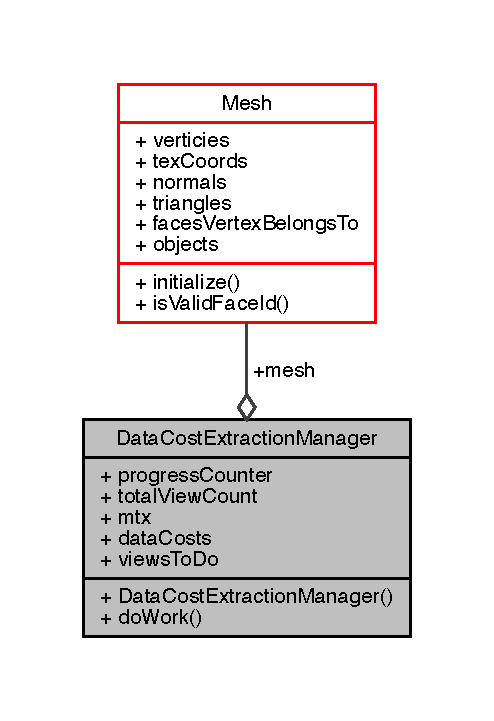
\includegraphics[width=237pt]{class_data_cost_extraction_manager__coll__graph}
\end{center}
\end{figure}
\subsection*{Public Member Functions}
\begin{DoxyCompactItemize}
\item 
\hyperlink{class_data_cost_extraction_manager_a90368fe041fe99c6ee45531ca69ae036}{Data\+Cost\+Extraction\+Manager} (const \hyperlink{class_mesh}{Mesh} \&\hyperlink{class_data_cost_extraction_manager_afa915680af20f1ac535cbc3205f7c35a}{mesh})
\item 
void \hyperlink{class_data_cost_extraction_manager_a078e39ed154e6337584a2506a87c35e7}{do\+Work} ()
\end{DoxyCompactItemize}
\subsection*{Public Attributes}
\begin{DoxyCompactItemize}
\item 
uint $\ast$ \hyperlink{class_data_cost_extraction_manager_a97997e576d25554a8805934a81382d38}{progress\+Counter}
\item 
uint \hyperlink{class_data_cost_extraction_manager_ad2cbdefd98fdde78bf62b5602befa9e5}{total\+View\+Count}
\item 
const \hyperlink{class_mesh}{Mesh} \& \hyperlink{class_data_cost_extraction_manager_afa915680af20f1ac535cbc3205f7c35a}{mesh}
\item 
std\+::mutex $\ast$ \hyperlink{class_data_cost_extraction_manager_a701cc390cea498e7477cd2e06cf48e01}{mtx}
\item 
std\+::map$<$ uint, std\+::map$<$ uint, \hyperlink{struct_patch_quality}{Patch\+Quality} $>$ $>$ $\ast$ \hyperlink{class_data_cost_extraction_manager_aab34038a5dd8e8e24a44fe102e722cca}{data\+Costs}
\item 
std\+::vector$<$ \hyperlink{class_view}{View} $\ast$ $>$ \hyperlink{class_data_cost_extraction_manager_afec2fa6aa627fb80c2734b4c5f895afa}{views\+To\+Do}
\end{DoxyCompactItemize}


\subsection{Detailed Description}
Class that is responsible for keeping track of the workload and performs the main thread loop in the do\+Work method, and a \hyperlink{class_data_costs_extractor}{Data\+Costs\+Extractor} class perform an extraction for one source image itself. 

\subsection{Constructor \& Destructor Documentation}
\hypertarget{class_data_cost_extraction_manager_a90368fe041fe99c6ee45531ca69ae036}{}\index{Data\+Cost\+Extraction\+Manager@{Data\+Cost\+Extraction\+Manager}!Data\+Cost\+Extraction\+Manager@{Data\+Cost\+Extraction\+Manager}}
\index{Data\+Cost\+Extraction\+Manager@{Data\+Cost\+Extraction\+Manager}!Data\+Cost\+Extraction\+Manager@{Data\+Cost\+Extraction\+Manager}}
\subsubsection[{Data\+Cost\+Extraction\+Manager(const Mesh \&mesh)}]{\setlength{\rightskip}{0pt plus 5cm}Data\+Cost\+Extraction\+Manager\+::\+Data\+Cost\+Extraction\+Manager (
\begin{DoxyParamCaption}
\item[{const {\bf Mesh} \&}]{mesh}
\end{DoxyParamCaption}
)\hspace{0.3cm}{\ttfamily [inline]}}\label{class_data_cost_extraction_manager_a90368fe041fe99c6ee45531ca69ae036}


\subsection{Member Function Documentation}
\hypertarget{class_data_cost_extraction_manager_a078e39ed154e6337584a2506a87c35e7}{}\index{Data\+Cost\+Extraction\+Manager@{Data\+Cost\+Extraction\+Manager}!do\+Work@{do\+Work}}
\index{do\+Work@{do\+Work}!Data\+Cost\+Extraction\+Manager@{Data\+Cost\+Extraction\+Manager}}
\subsubsection[{do\+Work()}]{\setlength{\rightskip}{0pt plus 5cm}void Data\+Cost\+Extraction\+Manager\+::do\+Work (
\begin{DoxyParamCaption}
{}
\end{DoxyParamCaption}
)}\label{class_data_cost_extraction_manager_a078e39ed154e6337584a2506a87c35e7}
Main function that is called in the begging of the thread 

\subsection{Member Data Documentation}
\hypertarget{class_data_cost_extraction_manager_aab34038a5dd8e8e24a44fe102e722cca}{}\index{Data\+Cost\+Extraction\+Manager@{Data\+Cost\+Extraction\+Manager}!data\+Costs@{data\+Costs}}
\index{data\+Costs@{data\+Costs}!Data\+Cost\+Extraction\+Manager@{Data\+Cost\+Extraction\+Manager}}
\subsubsection[{data\+Costs}]{\setlength{\rightskip}{0pt plus 5cm}std\+::map$<$uint,std\+::map$<$uint,{\bf Patch\+Quality}$>$ $>$$\ast$ Data\+Cost\+Extraction\+Manager\+::data\+Costs}\label{class_data_cost_extraction_manager_aab34038a5dd8e8e24a44fe102e722cca}
Set of data costs for every triangle visible from one particular source image. Those sets are combined into one data\+Costs set local to a \hyperlink{class_data_cost_extraction_manager}{Data\+Cost\+Extraction\+Manager}. This means, that since we have as many Data\+Cost\+Extraction\+Managers as threads, we have to later merge them. \hypertarget{class_data_cost_extraction_manager_afa915680af20f1ac535cbc3205f7c35a}{}\index{Data\+Cost\+Extraction\+Manager@{Data\+Cost\+Extraction\+Manager}!mesh@{mesh}}
\index{mesh@{mesh}!Data\+Cost\+Extraction\+Manager@{Data\+Cost\+Extraction\+Manager}}
\subsubsection[{mesh}]{\setlength{\rightskip}{0pt plus 5cm}const {\bf Mesh}\& Data\+Cost\+Extraction\+Manager\+::mesh}\label{class_data_cost_extraction_manager_afa915680af20f1ac535cbc3205f7c35a}
Work mesh \hypertarget{class_data_cost_extraction_manager_a701cc390cea498e7477cd2e06cf48e01}{}\index{Data\+Cost\+Extraction\+Manager@{Data\+Cost\+Extraction\+Manager}!mtx@{mtx}}
\index{mtx@{mtx}!Data\+Cost\+Extraction\+Manager@{Data\+Cost\+Extraction\+Manager}}
\subsubsection[{mtx}]{\setlength{\rightskip}{0pt plus 5cm}std\+::mutex$\ast$ Data\+Cost\+Extraction\+Manager\+::mtx}\label{class_data_cost_extraction_manager_a701cc390cea498e7477cd2e06cf48e01}
Common mutex between extraction managers. U\+Sed to report the progress \hypertarget{class_data_cost_extraction_manager_a97997e576d25554a8805934a81382d38}{}\index{Data\+Cost\+Extraction\+Manager@{Data\+Cost\+Extraction\+Manager}!progress\+Counter@{progress\+Counter}}
\index{progress\+Counter@{progress\+Counter}!Data\+Cost\+Extraction\+Manager@{Data\+Cost\+Extraction\+Manager}}
\subsubsection[{progress\+Counter}]{\setlength{\rightskip}{0pt plus 5cm}uint$\ast$ Data\+Cost\+Extraction\+Manager\+::progress\+Counter}\label{class_data_cost_extraction_manager_a97997e576d25554a8805934a81382d38}
Counter for keeping track of progress. is shared between parallel mangaers. Gets incremented i nthe mutex protected part. \hypertarget{class_data_cost_extraction_manager_ad2cbdefd98fdde78bf62b5602befa9e5}{}\index{Data\+Cost\+Extraction\+Manager@{Data\+Cost\+Extraction\+Manager}!total\+View\+Count@{total\+View\+Count}}
\index{total\+View\+Count@{total\+View\+Count}!Data\+Cost\+Extraction\+Manager@{Data\+Cost\+Extraction\+Manager}}
\subsubsection[{total\+View\+Count}]{\setlength{\rightskip}{0pt plus 5cm}uint Data\+Cost\+Extraction\+Manager\+::total\+View\+Count}\label{class_data_cost_extraction_manager_ad2cbdefd98fdde78bf62b5602befa9e5}
Tottal number of views a mangager has to analyze. It is its workload \hypertarget{class_data_cost_extraction_manager_afec2fa6aa627fb80c2734b4c5f895afa}{}\index{Data\+Cost\+Extraction\+Manager@{Data\+Cost\+Extraction\+Manager}!views\+To\+Do@{views\+To\+Do}}
\index{views\+To\+Do@{views\+To\+Do}!Data\+Cost\+Extraction\+Manager@{Data\+Cost\+Extraction\+Manager}}
\subsubsection[{views\+To\+Do}]{\setlength{\rightskip}{0pt plus 5cm}std\+::vector$<${\bf View} $\ast$$>$ Data\+Cost\+Extraction\+Manager\+::views\+To\+Do}\label{class_data_cost_extraction_manager_afec2fa6aa627fb80c2734b4c5f895afa}
List of views a managher should do. It is its workload 

The documentation for this class was generated from the following files\+:\begin{DoxyCompactItemize}
\item 
Texture\+Extractor\+V2/\hyperlink{_data_cost_extraction_manager_8hpp}{Data\+Cost\+Extraction\+Manager.\+hpp}\item 
Texture\+Extractor\+V2/\hyperlink{_data_cost_extraction_manager_8cpp}{Data\+Cost\+Extraction\+Manager.\+cpp}\end{DoxyCompactItemize}

\hypertarget{class_data_costs_extractor}{}\section{Data\+Costs\+Extractor Class Reference}
\label{class_data_costs_extractor}\index{Data\+Costs\+Extractor@{Data\+Costs\+Extractor}}
\subsection*{Public Member Functions}
\begin{DoxyCompactItemize}
\item 
\hypertarget{class_data_costs_extractor_a43e088a660a4c58abe525cae2fb6925b}{}{\bfseries Data\+Costs\+Extractor} (const \hyperlink{class_mesh}{Mesh} \&mesh, \hyperlink{class_view}{View} \&view)\label{class_data_costs_extractor_a43e088a660a4c58abe525cae2fb6925b}

\item 
\hypertarget{class_data_costs_extractor_a7c072ab9a7ceb6e3c6742c9991923b00}{}std\+::map$<$ uint, \hyperlink{struct_patch_quality}{Patch\+Quality} $>$ {\bfseries calculate\+Costs} ()\label{class_data_costs_extractor_a7c072ab9a7ceb6e3c6742c9991923b00}

\end{DoxyCompactItemize}


The documentation for this class was generated from the following files\+:\begin{DoxyCompactItemize}
\item 
Texture\+Extractor\+V2/Data\+Costs\+Extractor.\+hpp\item 
Texture\+Extractor\+V2/Data\+Costs\+Extractor.\+cpp\end{DoxyCompactItemize}

\hypertarget{class_edge}{}\section{Edge Class Reference}
\label{class_edge}\index{Edge@{Edge}}
\subsection*{Public Member Functions}
\begin{DoxyCompactItemize}
\item 
\hypertarget{class_edge_a97a820beb3ce7430825616b227189845}{}{\bfseries Edge} (\hyperlink{struct_vertex}{Vertex} start, \hyperlink{struct_vertex}{Vertex} end, \hyperlink{class_gradient}{Gradient} gradient, int min\+Y\+Vert\+Index)\label{class_edge_a97a820beb3ce7430825616b227189845}

\item 
\hypertarget{class_edge_aee421bbd01b0ac8006e91e76589e84fb}{}void {\bfseries Step} ()\label{class_edge_aee421bbd01b0ac8006e91e76589e84fb}

\end{DoxyCompactItemize}
\subsection*{Public Attributes}
\begin{DoxyCompactItemize}
\item 
\hypertarget{class_edge_a23bac6cf22ad265c83e42219b548f199}{}float {\bfseries current\+X}\label{class_edge_a23bac6cf22ad265c83e42219b548f199}

\item 
\hypertarget{class_edge_a56c4a79ba0032fb252f68d30a7374f53}{}float {\bfseries x\+Step}\label{class_edge_a56c4a79ba0032fb252f68d30a7374f53}

\item 
\hypertarget{class_edge_a647499228d18f2e4955d1ebe98221e08}{}float {\bfseries y\+Start}\label{class_edge_a647499228d18f2e4955d1ebe98221e08}

\item 
\hypertarget{class_edge_a588e6a6d5a5caf93d541dc0db2d9103f}{}float {\bfseries y\+End}\label{class_edge_a588e6a6d5a5caf93d541dc0db2d9103f}

\item 
\hypertarget{class_edge_a7584501b6ec92a63e26dbbb2cfec8329}{}glm\+::vec4 {\bfseries color}\label{class_edge_a7584501b6ec92a63e26dbbb2cfec8329}

\item 
\hypertarget{class_edge_ab62623a8423d759cc44d45131f74ac6c}{}glm\+::vec4 {\bfseries color\+Step}\label{class_edge_ab62623a8423d759cc44d45131f74ac6c}

\item 
\hypertarget{class_edge_a183c69d2816a58570695cde3c3e73a8d}{}float {\bfseries one\+Over\+Z}\label{class_edge_a183c69d2816a58570695cde3c3e73a8d}

\item 
\hypertarget{class_edge_adee1d668c241bfc0dbad1637b07f2893}{}float {\bfseries one\+Over\+Z\+Step}\label{class_edge_adee1d668c241bfc0dbad1637b07f2893}

\item 
\hypertarget{class_edge_a997c97e02df725e1397a5e2fe4c573f3}{}float {\bfseries depth}\label{class_edge_a997c97e02df725e1397a5e2fe4c573f3}

\item 
\hypertarget{class_edge_ae85a7f75238e8212db2f1fc90729afcd}{}float {\bfseries depth\+Step}\label{class_edge_ae85a7f75238e8212db2f1fc90729afcd}

\item 
\hypertarget{class_edge_ac60ac724a2206426daeefa8781f1bef8}{}glm\+::vec2 {\bfseries tex\+Coord}\label{class_edge_ac60ac724a2206426daeefa8781f1bef8}

\item 
\hypertarget{class_edge_ab18d6715948ccf609e0b40f48349b533}{}glm\+::vec2 {\bfseries tex\+Coord\+Step}\label{class_edge_ab18d6715948ccf609e0b40f48349b533}

\end{DoxyCompactItemize}


The documentation for this class was generated from the following files\+:\begin{DoxyCompactItemize}
\item 
Texture\+Extractor\+V2/Edge.\+hpp\item 
Texture\+Extractor\+V2/Edge.\+cpp\end{DoxyCompactItemize}

\hypertarget{struct_edge_vertex}{}\section{Edge\+Vertex Struct Reference}
\label{struct_edge_vertex}\index{Edge\+Vertex@{Edge\+Vertex}}
\subsection*{Public Attributes}
\begin{DoxyCompactItemize}
\item 
\hypertarget{struct_edge_vertex_a8439c6928189921562f355db598fcf01}{}uint {\bfseries common\+Vertex}\label{struct_edge_vertex_a8439c6928189921562f355db598fcf01}

\item 
\hypertarget{struct_edge_vertex_a0383800c9299c747dc5ddbf4b397806d}{}uint {\bfseries neighbour\+I\+D}\label{struct_edge_vertex_a0383800c9299c747dc5ddbf4b397806d}

\item 
\hypertarget{struct_edge_vertex_a7c1790b8527e54c9eca13038c5351032}{}glm\+::vec4 {\bfseries color\+Diff}\label{struct_edge_vertex_a7c1790b8527e54c9eca13038c5351032}

\end{DoxyCompactItemize}


The documentation for this struct was generated from the following file\+:\begin{DoxyCompactItemize}
\item 
Texture\+Extractor\+V2/Texture\+Patch.\+hpp\end{DoxyCompactItemize}

\hypertarget{class_extraction_worker}{}\section{Extraction\+Worker Class Reference}
\label{class_extraction_worker}\index{Extraction\+Worker@{Extraction\+Worker}}


{\ttfamily \#include $<$Extraction\+Worker.\+hpp$>$}

\subsection*{Public Member Functions}
\begin{DoxyCompactItemize}
\item 
\hypertarget{class_extraction_worker_a5cb5231da6a9c3568c1cbdeaa90a30e2}{}{\bfseries Extraction\+Worker} (const \hyperlink{class_mesh}{Mesh} $\ast$mesh)\label{class_extraction_worker_a5cb5231da6a9c3568c1cbdeaa90a30e2}

\item 
void \hyperlink{class_extraction_worker_ad649a3ebbc506e55d5b003381b07ba06}{extract} (\hyperlink{struct_triangle}{Triangle} face, \hyperlink{class_bitmap}{Bitmap} \&tex, \hyperlink{class_view}{View} \&view)
\item 
void \hyperlink{class_extraction_worker_a24312158a7768088b96dd722414786ae}{extend} (\hyperlink{struct_triangle}{Triangle} face, \hyperlink{class_bitmap}{Bitmap} \&tex)
\item 
void \hyperlink{class_extraction_worker_ac956797cff498d82f040d3884be2144d}{apply\+Gradient} (\hyperlink{struct_triangle}{Triangle} face, \hyperlink{class_bitmap}{Bitmap} \&src, \hyperlink{class_bitmap}{Bitmap} \&dst, glm\+::vec4 color\mbox{[}3\mbox{]}, \hyperlink{class_bitmap}{Bitmap} \&leveling\+Texture)
\item 
void \hyperlink{class_extraction_worker_a3ae8fdacd8e2a0b44873c36b6e3756e5}{set\+Mask} (\hyperlink{class_bitmap}{Bitmap} $\ast$m)
\item 
void \hyperlink{class_extraction_worker_a0bfb06fd0caed6ec032416e8d928fbe8}{set\+Mesh} (const \hyperlink{class_mesh}{Mesh} $\ast$m)
\item 
void \hyperlink{class_extraction_worker_a25d7438c2adfc4e4e4076954516a4f43}{fill\+Texture\+Triangle} (\hyperlink{struct_triangle}{Triangle} face, glm\+::vec4 color, \hyperlink{class_bitmap}{Bitmap} \&destination)
\end{DoxyCompactItemize}


\subsection{Detailed Description}
Worker class. Extracts texture information from a photographs. 

\subsection{Member Function Documentation}
\hypertarget{class_extraction_worker_ac956797cff498d82f040d3884be2144d}{}\index{Extraction\+Worker@{Extraction\+Worker}!apply\+Gradient@{apply\+Gradient}}
\index{apply\+Gradient@{apply\+Gradient}!Extraction\+Worker@{Extraction\+Worker}}
\subsubsection[{apply\+Gradient(\+Triangle face, Bitmap \&src, Bitmap \&dst, glm\+::vec4 color[3], Bitmap \&leveling\+Texture)}]{\setlength{\rightskip}{0pt plus 5cm}void Extraction\+Worker\+::apply\+Gradient (
\begin{DoxyParamCaption}
\item[{{\bf Triangle}}]{face, }
\item[{{\bf Bitmap} \&}]{src, }
\item[{{\bf Bitmap} \&}]{dst, }
\item[{glm\+::vec4}]{color\mbox{[}3\mbox{]}, }
\item[{{\bf Bitmap} \&}]{leveling\+Texture}
\end{DoxyParamCaption}
)}\label{class_extraction_worker_ac956797cff498d82f040d3884be2144d}
Applies a gradient to a texture triangle 
\begin{DoxyParams}{Parameters}
{\em face} & target triangle \\
\hline
{\em dst} & output texture \\
\hline
{\em src} & texture for initial sampling \\
\hline
{\em color} & set of color adjustment gradients for every vertex. \\
\hline
{\em output} & leveling texture \\
\hline
{\em view} & source view \\
\hline
\end{DoxyParams}
\hypertarget{class_extraction_worker_a24312158a7768088b96dd722414786ae}{}\index{Extraction\+Worker@{Extraction\+Worker}!extend@{extend}}
\index{extend@{extend}!Extraction\+Worker@{Extraction\+Worker}}
\subsubsection[{extend(\+Triangle face, Bitmap \&tex)}]{\setlength{\rightskip}{0pt plus 5cm}void Extraction\+Worker\+::extend (
\begin{DoxyParamCaption}
\item[{{\bf Triangle}}]{face, }
\item[{{\bf Bitmap} \&}]{tex}
\end{DoxyParamCaption}
)}\label{class_extraction_worker_a24312158a7768088b96dd722414786ae}
Starts an extension on a texture triangle 
\begin{DoxyParams}{Parameters}
{\em face} & target triangle \\
\hline
{\em tex} & output texture \\
\hline
\end{DoxyParams}
\hypertarget{class_extraction_worker_ad649a3ebbc506e55d5b003381b07ba06}{}\index{Extraction\+Worker@{Extraction\+Worker}!extract@{extract}}
\index{extract@{extract}!Extraction\+Worker@{Extraction\+Worker}}
\subsubsection[{extract(\+Triangle face, Bitmap \&tex, View \&view)}]{\setlength{\rightskip}{0pt plus 5cm}void Extraction\+Worker\+::extract (
\begin{DoxyParamCaption}
\item[{{\bf Triangle}}]{face, }
\item[{{\bf Bitmap} \&}]{tex, }
\item[{{\bf View} \&}]{view}
\end{DoxyParamCaption}
)}\label{class_extraction_worker_ad649a3ebbc506e55d5b003381b07ba06}
Starts an extraction process for one trinagle 
\begin{DoxyParams}{Parameters}
{\em face} & target triangle \\
\hline
{\em tex} & output texture \\
\hline
{\em view} & source view \\
\hline
\end{DoxyParams}
\hypertarget{class_extraction_worker_a25d7438c2adfc4e4e4076954516a4f43}{}\index{Extraction\+Worker@{Extraction\+Worker}!fill\+Texture\+Triangle@{fill\+Texture\+Triangle}}
\index{fill\+Texture\+Triangle@{fill\+Texture\+Triangle}!Extraction\+Worker@{Extraction\+Worker}}
\subsubsection[{fill\+Texture\+Triangle(\+Triangle face, glm\+::vec4 color, Bitmap \&destination)}]{\setlength{\rightskip}{0pt plus 5cm}void Extraction\+Worker\+::fill\+Texture\+Triangle (
\begin{DoxyParamCaption}
\item[{{\bf Triangle}}]{face, }
\item[{glm\+::vec4}]{color, }
\item[{{\bf Bitmap} \&}]{destination}
\end{DoxyParamCaption}
)}\label{class_extraction_worker_a25d7438c2adfc4e4e4076954516a4f43}
Fills a texture triangle with solid color 
\begin{DoxyParams}{Parameters}
{\em face} & target triangle \\
\hline
{\em destination} & output texture \\
\hline
{\em color} & a color to applye \\
\hline
\end{DoxyParams}
\hypertarget{class_extraction_worker_a3ae8fdacd8e2a0b44873c36b6e3756e5}{}\index{Extraction\+Worker@{Extraction\+Worker}!set\+Mask@{set\+Mask}}
\index{set\+Mask@{set\+Mask}!Extraction\+Worker@{Extraction\+Worker}}
\subsubsection[{set\+Mask(\+Bitmap $\ast$m)}]{\setlength{\rightskip}{0pt plus 5cm}void Extraction\+Worker\+::set\+Mask (
\begin{DoxyParamCaption}
\item[{{\bf Bitmap} $\ast$}]{m}
\end{DoxyParamCaption}
)\hspace{0.3cm}{\ttfamily [inline]}}\label{class_extraction_worker_a3ae8fdacd8e2a0b44873c36b6e3756e5}
Sets a new bloking mask 
\begin{DoxyParams}{Parameters}
{\em m} & new mask \\
\hline
\end{DoxyParams}
\hypertarget{class_extraction_worker_a0bfb06fd0caed6ec032416e8d928fbe8}{}\index{Extraction\+Worker@{Extraction\+Worker}!set\+Mesh@{set\+Mesh}}
\index{set\+Mesh@{set\+Mesh}!Extraction\+Worker@{Extraction\+Worker}}
\subsubsection[{set\+Mesh(const Mesh $\ast$m)}]{\setlength{\rightskip}{0pt plus 5cm}void Extraction\+Worker\+::set\+Mesh (
\begin{DoxyParamCaption}
\item[{const {\bf Mesh} $\ast$}]{m}
\end{DoxyParamCaption}
)\hspace{0.3cm}{\ttfamily [inline]}}\label{class_extraction_worker_a0bfb06fd0caed6ec032416e8d928fbe8}
Sets a working mesh 
\begin{DoxyParams}{Parameters}
{\em m} & a mesh \\
\hline
\end{DoxyParams}


The documentation for this class was generated from the following files\+:\begin{DoxyCompactItemize}
\item 
Texture\+Extractor\+V2/Extraction\+Worker.\+hpp\item 
Texture\+Extractor\+V2/Extraction\+Worker\+\_\+apply\+Gradient.\+cpp\item 
Texture\+Extractor\+V2/Extraction\+Worker\+\_\+common\+Code.\+cpp\item 
Texture\+Extractor\+V2/Extraction\+Worker\+\_\+extend.\+cpp\item 
Texture\+Extractor\+V2/Extraction\+Worker\+\_\+extract.\+cpp\item 
Texture\+Extractor\+V2/Extraction\+Worker\+\_\+fill\+Texture\+Triangle\+Color.\+cpp\end{DoxyCompactItemize}

\hypertarget{class_gradient}{}\section{Gradient Class Reference}
\label{class_gradient}\index{Gradient@{Gradient}}


{\ttfamily \#include $<$Gradient.\+hpp$>$}



Collaboration diagram for Gradient\+:\nopagebreak
\begin{figure}[H]
\begin{center}
\leavevmode
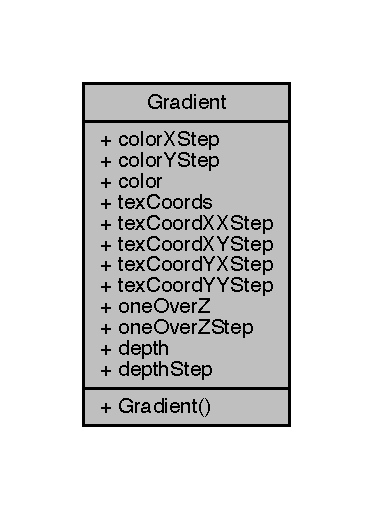
\includegraphics[width=179pt]{class_gradient__coll__graph}
\end{center}
\end{figure}
\subsection*{Public Member Functions}
\begin{DoxyCompactItemize}
\item 
\hyperlink{class_gradient_a4fd340dfd44bc432746d239cb809a0ee}{Gradient} (\hyperlink{struct_vertex}{Vertex} min\+Y\+Vert, \hyperlink{struct_vertex}{Vertex} mid\+Y\+Vert, \hyperlink{struct_vertex}{Vertex} max\+Y\+Vert)
\end{DoxyCompactItemize}
\subsection*{Public Attributes}
\begin{DoxyCompactItemize}
\item 
glm\+::vec4 \hyperlink{class_gradient_a0451719335035c075a67204cdb80252f}{color\+X\+Step}
\item 
glm\+::vec4 \hyperlink{class_gradient_a3ac810ca548605633dd2497d9376e583}{color\+Y\+Step}
\item 
glm\+::vec4 \hyperlink{class_gradient_a71c3ddc8c7826a17338723232d9bc7ea}{color} \mbox{[}3\mbox{]}
\item 
glm\+::vec2 \hyperlink{class_gradient_ae71837d2a5b35d006054d5d474eddb1a}{tex\+Coords} \mbox{[}3\mbox{]}
\item 
float \hyperlink{class_gradient_a624a5bc1117ef0ff5586505bd7414b00}{tex\+Coord\+X\+X\+Step}
\item 
float \hyperlink{class_gradient_a8afadd4049d8b9eb22cbc400e70560aa}{tex\+Coord\+X\+Y\+Step}
\item 
float \hyperlink{class_gradient_a81d975aa437d9aa2d4f4902073c1f529}{tex\+Coord\+Y\+X\+Step}
\item 
float \hyperlink{class_gradient_a7d935258d173da77270987a4c95f3462}{tex\+Coord\+Y\+Y\+Step}
\item 
float \hyperlink{class_gradient_aab07e150dbcc6550c252b66180ceceb2}{one\+Over\+Z} \mbox{[}3\mbox{]}
\item 
glm\+::vec2 \hyperlink{class_gradient_aa3bc11489f5f615cafc9dc8c8c180145}{one\+Over\+Z\+Step}
\item 
float \hyperlink{class_gradient_ac0077f281e1539333e984574e8f728a3}{depth} \mbox{[}3\mbox{]}
\item 
glm\+::vec2 \hyperlink{class_gradient_a45a2e551be6a31ce12fdc3c39191914f}{depth\+Step}
\end{DoxyCompactItemize}


\subsection{Detailed Description}
Class that sets up a interpolation gradient 

\subsection{Constructor \& Destructor Documentation}
\hypertarget{class_gradient_a4fd340dfd44bc432746d239cb809a0ee}{}\index{Gradient@{Gradient}!Gradient@{Gradient}}
\index{Gradient@{Gradient}!Gradient@{Gradient}}
\subsubsection[{Gradient(\+Vertex min\+Y\+Vert, Vertex mid\+Y\+Vert, Vertex max\+Y\+Vert)}]{\setlength{\rightskip}{0pt plus 5cm}Gradient\+::\+Gradient (
\begin{DoxyParamCaption}
\item[{{\bf Vertex}}]{min\+Y\+Vert, }
\item[{{\bf Vertex}}]{mid\+Y\+Vert, }
\item[{{\bf Vertex}}]{max\+Y\+Vert}
\end{DoxyParamCaption}
)}\label{class_gradient_a4fd340dfd44bc432746d239cb809a0ee}
Sets up a gradient. Uses three verticies to acalculate steppin values. depth 

\subsection{Member Data Documentation}
\hypertarget{class_gradient_a71c3ddc8c7826a17338723232d9bc7ea}{}\index{Gradient@{Gradient}!color@{color}}
\index{color@{color}!Gradient@{Gradient}}
\subsubsection[{color}]{\setlength{\rightskip}{0pt plus 5cm}glm\+::vec4 Gradient\+::color\mbox{[}3\mbox{]}}\label{class_gradient_a71c3ddc8c7826a17338723232d9bc7ea}
Color values at the verticies that make up gradient \hypertarget{class_gradient_a0451719335035c075a67204cdb80252f}{}\index{Gradient@{Gradient}!color\+X\+Step@{color\+X\+Step}}
\index{color\+X\+Step@{color\+X\+Step}!Gradient@{Gradient}}
\subsubsection[{color\+X\+Step}]{\setlength{\rightskip}{0pt plus 5cm}glm\+::vec4 Gradient\+::color\+X\+Step}\label{class_gradient_a0451719335035c075a67204cdb80252f}
Color step as we move in the x direction \hypertarget{class_gradient_a3ac810ca548605633dd2497d9376e583}{}\index{Gradient@{Gradient}!color\+Y\+Step@{color\+Y\+Step}}
\index{color\+Y\+Step@{color\+Y\+Step}!Gradient@{Gradient}}
\subsubsection[{color\+Y\+Step}]{\setlength{\rightskip}{0pt plus 5cm}glm\+::vec4 Gradient\+::color\+Y\+Step}\label{class_gradient_a3ac810ca548605633dd2497d9376e583}
Color step as we move in the y direction \hypertarget{class_gradient_ac0077f281e1539333e984574e8f728a3}{}\index{Gradient@{Gradient}!depth@{depth}}
\index{depth@{depth}!Gradient@{Gradient}}
\subsubsection[{depth}]{\setlength{\rightskip}{0pt plus 5cm}float Gradient\+::depth\mbox{[}3\mbox{]}}\label{class_gradient_ac0077f281e1539333e984574e8f728a3}
Depth value at the verticies that make up gradient \hypertarget{class_gradient_a45a2e551be6a31ce12fdc3c39191914f}{}\index{Gradient@{Gradient}!depth\+Step@{depth\+Step}}
\index{depth\+Step@{depth\+Step}!Gradient@{Gradient}}
\subsubsection[{depth\+Step}]{\setlength{\rightskip}{0pt plus 5cm}glm\+::vec2 Gradient\+::depth\+Step}\label{class_gradient_a45a2e551be6a31ce12fdc3c39191914f}
Depth step step \hypertarget{class_gradient_aab07e150dbcc6550c252b66180ceceb2}{}\index{Gradient@{Gradient}!one\+Over\+Z@{one\+Over\+Z}}
\index{one\+Over\+Z@{one\+Over\+Z}!Gradient@{Gradient}}
\subsubsection[{one\+Over\+Z}]{\setlength{\rightskip}{0pt plus 5cm}float Gradient\+::one\+Over\+Z\mbox{[}3\mbox{]}}\label{class_gradient_aab07e150dbcc6550c252b66180ceceb2}
One over z at the verticies that make up gradient \hypertarget{class_gradient_aa3bc11489f5f615cafc9dc8c8c180145}{}\index{Gradient@{Gradient}!one\+Over\+Z\+Step@{one\+Over\+Z\+Step}}
\index{one\+Over\+Z\+Step@{one\+Over\+Z\+Step}!Gradient@{Gradient}}
\subsubsection[{one\+Over\+Z\+Step}]{\setlength{\rightskip}{0pt plus 5cm}glm\+::vec2 Gradient\+::one\+Over\+Z\+Step}\label{class_gradient_aa3bc11489f5f615cafc9dc8c8c180145}
One over\+Z step \hypertarget{class_gradient_ae71837d2a5b35d006054d5d474eddb1a}{}\index{Gradient@{Gradient}!tex\+Coords@{tex\+Coords}}
\index{tex\+Coords@{tex\+Coords}!Gradient@{Gradient}}
\subsubsection[{tex\+Coords}]{\setlength{\rightskip}{0pt plus 5cm}glm\+::vec2 Gradient\+::tex\+Coords\mbox{[}3\mbox{]}}\label{class_gradient_ae71837d2a5b35d006054d5d474eddb1a}
Texture coordinates at the verticies that make up gradient \hypertarget{class_gradient_a624a5bc1117ef0ff5586505bd7414b00}{}\index{Gradient@{Gradient}!tex\+Coord\+X\+X\+Step@{tex\+Coord\+X\+X\+Step}}
\index{tex\+Coord\+X\+X\+Step@{tex\+Coord\+X\+X\+Step}!Gradient@{Gradient}}
\subsubsection[{tex\+Coord\+X\+X\+Step}]{\setlength{\rightskip}{0pt plus 5cm}float Gradient\+::tex\+Coord\+X\+X\+Step}\label{class_gradient_a624a5bc1117ef0ff5586505bd7414b00}
Texture coordinate x step as we move in the x direction on a raster \hypertarget{class_gradient_a8afadd4049d8b9eb22cbc400e70560aa}{}\index{Gradient@{Gradient}!tex\+Coord\+X\+Y\+Step@{tex\+Coord\+X\+Y\+Step}}
\index{tex\+Coord\+X\+Y\+Step@{tex\+Coord\+X\+Y\+Step}!Gradient@{Gradient}}
\subsubsection[{tex\+Coord\+X\+Y\+Step}]{\setlength{\rightskip}{0pt plus 5cm}float Gradient\+::tex\+Coord\+X\+Y\+Step}\label{class_gradient_a8afadd4049d8b9eb22cbc400e70560aa}
Texture coordinate x step as we move in the y direction on a raster \hypertarget{class_gradient_a81d975aa437d9aa2d4f4902073c1f529}{}\index{Gradient@{Gradient}!tex\+Coord\+Y\+X\+Step@{tex\+Coord\+Y\+X\+Step}}
\index{tex\+Coord\+Y\+X\+Step@{tex\+Coord\+Y\+X\+Step}!Gradient@{Gradient}}
\subsubsection[{tex\+Coord\+Y\+X\+Step}]{\setlength{\rightskip}{0pt plus 5cm}float Gradient\+::tex\+Coord\+Y\+X\+Step}\label{class_gradient_a81d975aa437d9aa2d4f4902073c1f529}
Texture coordinate y step as we move in the x direction on a raster \hypertarget{class_gradient_a7d935258d173da77270987a4c95f3462}{}\index{Gradient@{Gradient}!tex\+Coord\+Y\+Y\+Step@{tex\+Coord\+Y\+Y\+Step}}
\index{tex\+Coord\+Y\+Y\+Step@{tex\+Coord\+Y\+Y\+Step}!Gradient@{Gradient}}
\subsubsection[{tex\+Coord\+Y\+Y\+Step}]{\setlength{\rightskip}{0pt plus 5cm}float Gradient\+::tex\+Coord\+Y\+Y\+Step}\label{class_gradient_a7d935258d173da77270987a4c95f3462}
Texture coordinate y step as we move in the y direction on a raster 

The documentation for this class was generated from the following files\+:\begin{DoxyCompactItemize}
\item 
Texture\+Extractor\+V2/\hyperlink{_gradient_8hpp}{Gradient.\+hpp}\item 
Texture\+Extractor\+V2/\hyperlink{_gradient_8cpp}{Gradient.\+cpp}\end{DoxyCompactItemize}

\hypertarget{class_i_n_i_reader}{}\section{I\+N\+I\+Reader Class Reference}
\label{class_i_n_i_reader}\index{I\+N\+I\+Reader@{I\+N\+I\+Reader}}
\subsection*{Public Member Functions}
\begin{DoxyCompactItemize}
\item 
\hypertarget{class_i_n_i_reader_a357e21f6b1bc10b17bd3a7b72452cb57}{}{\bfseries I\+N\+I\+Reader} (std\+::string filename)\label{class_i_n_i_reader_a357e21f6b1bc10b17bd3a7b72452cb57}

\item 
\hypertarget{class_i_n_i_reader_aa40b260538dc123ef43fd07d86f0b729}{}int {\bfseries Parse\+Error} () const \label{class_i_n_i_reader_aa40b260538dc123ef43fd07d86f0b729}

\item 
\hypertarget{class_i_n_i_reader_a8dc6b10ba3415f3c30c30c4fc342d867}{}std\+::set$<$ std\+::string $>$ {\bfseries Sections} ()\label{class_i_n_i_reader_a8dc6b10ba3415f3c30c30c4fc342d867}

\item 
\hypertarget{class_i_n_i_reader_a1042bfbb483afa305283a6f1a2bf27e9}{}std\+::string {\bfseries Get} (std\+::string section, std\+::string name, std\+::string default\+\_\+value)\label{class_i_n_i_reader_a1042bfbb483afa305283a6f1a2bf27e9}

\item 
\hypertarget{class_i_n_i_reader_a5fb288f961b8a43ba4974fbf97f4d1df}{}long {\bfseries Get\+Integer} (std\+::string section, std\+::string name, long default\+\_\+value)\label{class_i_n_i_reader_a5fb288f961b8a43ba4974fbf97f4d1df}

\item 
\hypertarget{class_i_n_i_reader_add45ae10b48fd12cb98a7b73e67d3a77}{}double {\bfseries Get\+Real} (std\+::string section, std\+::string name, double default\+\_\+value)\label{class_i_n_i_reader_add45ae10b48fd12cb98a7b73e67d3a77}

\item 
\hypertarget{class_i_n_i_reader_ac3d70858d357a6797b0d58a9a00d737e}{}bool {\bfseries Get\+Boolean} (std\+::string section, std\+::string name, bool default\+\_\+value)\label{class_i_n_i_reader_ac3d70858d357a6797b0d58a9a00d737e}

\end{DoxyCompactItemize}


The documentation for this class was generated from the following file\+:\begin{DoxyCompactItemize}
\item 
Texture\+Extractor\+V2/I\+N\+I\+Reader.\+h\end{DoxyCompactItemize}

\hypertarget{class_mesh}{}\section{Mesh Class Reference}
\label{class_mesh}\index{Mesh@{Mesh}}
\subsection*{Public Member Functions}
\begin{DoxyCompactItemize}
\item 
\hypertarget{class_mesh_ad93d51d3938b1fe01816746f7d6a121f}{}bool {\bfseries initialize} (const std\+::string \&filename)\label{class_mesh_ad93d51d3938b1fe01816746f7d6a121f}

\item 
\hypertarget{class_mesh_aaa92d27cfbbb7b2ae11d94ded72de982}{}bool {\bfseries is\+Valid\+Face\+Id} (int id)\label{class_mesh_aaa92d27cfbbb7b2ae11d94ded72de982}

\end{DoxyCompactItemize}
\subsection*{Public Attributes}
\begin{DoxyCompactItemize}
\item 
\hypertarget{class_mesh_a2cef656e11f17c6974a418c4fa0755fe}{}std\+::map$<$ uint, \hyperlink{struct_vertex}{Vertex} $>$ {\bfseries verticies}\label{class_mesh_a2cef656e11f17c6974a418c4fa0755fe}

\item 
\hypertarget{class_mesh_a615f86622e292b9bfa581cfad823b375}{}std\+::map$<$ uint, \hyperlink{struct_tex_coord}{Tex\+Coord} $>$ {\bfseries tex\+Coords}\label{class_mesh_a615f86622e292b9bfa581cfad823b375}

\item 
\hypertarget{class_mesh_afe59cf4410182ce7c42447b635c745e1}{}std\+::map$<$ uint, \hyperlink{struct_normal}{Normal} $>$ {\bfseries normals}\label{class_mesh_afe59cf4410182ce7c42447b635c745e1}

\item 
\hypertarget{class_mesh_a6afb31bd01dac6b21a548341d389b421}{}std\+::map$<$ uint, \hyperlink{struct_triangle}{Triangle} $>$ {\bfseries triangles}\label{class_mesh_a6afb31bd01dac6b21a548341d389b421}

\item 
\hypertarget{class_mesh_a5ad3c61ae2ecabc596a9d9cd01f29252}{}std\+::map$<$ uint, std\+::set$<$ uint $>$ $>$ {\bfseries faces\+Vertex\+Belongs\+To}\label{class_mesh_a5ad3c61ae2ecabc596a9d9cd01f29252}

\item 
\hypertarget{class_mesh_ad221985419bdc4e3f30396073e7aa107}{}std\+::vector$<$ \hyperlink{struct_object}{Object} $>$ {\bfseries objects}\label{class_mesh_ad221985419bdc4e3f30396073e7aa107}

\item 
\hypertarget{class_mesh_a7867e8a9f5b51b153a13d4e302578a1f}{}\hyperlink{class_adjacency_graph}{Adjacency\+Graph} {\bfseries adjacency\+Graph}\label{class_mesh_a7867e8a9f5b51b153a13d4e302578a1f}

\end{DoxyCompactItemize}


The documentation for this class was generated from the following files\+:\begin{DoxyCompactItemize}
\item 
Texture\+Extractor\+V2/Mesh.\+hpp\item 
Texture\+Extractor\+V2/Mesh.\+cpp\end{DoxyCompactItemize}

\hypertarget{struct_normal}{}\section{Normal Struct Reference}
\label{struct_normal}\index{Normal@{Normal}}


{\ttfamily \#include $<$Mesh.\+hpp$>$}



Collaboration diagram for Normal\+:\nopagebreak
\begin{figure}[H]
\begin{center}
\leavevmode
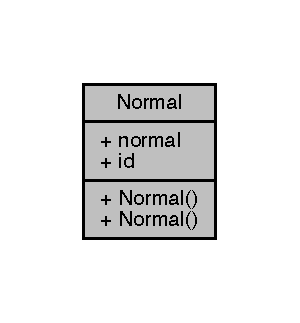
\includegraphics[width=144pt]{struct_normal__coll__graph}
\end{center}
\end{figure}
\subsection*{Public Member Functions}
\begin{DoxyCompactItemize}
\item 
\hyperlink{struct_normal_a19c72c824df84768e56cd6c610bf8edd}{Normal} (glm\+::vec4 coord)
\item 
\hyperlink{struct_normal_af62e51ec40dc2eedc3b9ca49ebdc7197}{Normal} ()
\end{DoxyCompactItemize}
\subsection*{Public Attributes}
\begin{DoxyCompactItemize}
\item 
glm\+::vec4 \hyperlink{struct_normal_a555de7ec7d67e743968b5f69af17dd1c}{normal}
\item 
uint \hyperlink{struct_normal_a39256c233377305342349bd73991d3e3}{id}
\end{DoxyCompactItemize}


\subsection{Detailed Description}
Structure that holds normal (not used in final tool) 

\subsection{Constructor \& Destructor Documentation}
\hypertarget{struct_normal_a19c72c824df84768e56cd6c610bf8edd}{}\index{Normal@{Normal}!Normal@{Normal}}
\index{Normal@{Normal}!Normal@{Normal}}
\subsubsection[{Normal(glm\+::vec4 coord)}]{\setlength{\rightskip}{0pt plus 5cm}Normal\+::\+Normal (
\begin{DoxyParamCaption}
\item[{glm\+::vec4}]{coord}
\end{DoxyParamCaption}
)\hspace{0.3cm}{\ttfamily [inline]}}\label{struct_normal_a19c72c824df84768e56cd6c610bf8edd}
\hypertarget{struct_normal_af62e51ec40dc2eedc3b9ca49ebdc7197}{}\index{Normal@{Normal}!Normal@{Normal}}
\index{Normal@{Normal}!Normal@{Normal}}
\subsubsection[{Normal()}]{\setlength{\rightskip}{0pt plus 5cm}Normal\+::\+Normal (
\begin{DoxyParamCaption}
{}
\end{DoxyParamCaption}
)\hspace{0.3cm}{\ttfamily [inline]}}\label{struct_normal_af62e51ec40dc2eedc3b9ca49ebdc7197}


\subsection{Member Data Documentation}
\hypertarget{struct_normal_a39256c233377305342349bd73991d3e3}{}\index{Normal@{Normal}!id@{id}}
\index{id@{id}!Normal@{Normal}}
\subsubsection[{id}]{\setlength{\rightskip}{0pt plus 5cm}uint Normal\+::id}\label{struct_normal_a39256c233377305342349bd73991d3e3}
normal I\+D \hypertarget{struct_normal_a555de7ec7d67e743968b5f69af17dd1c}{}\index{Normal@{Normal}!normal@{normal}}
\index{normal@{normal}!Normal@{Normal}}
\subsubsection[{normal}]{\setlength{\rightskip}{0pt plus 5cm}glm\+::vec4 Normal\+::normal}\label{struct_normal_a555de7ec7d67e743968b5f69af17dd1c}
normal vector 

The documentation for this struct was generated from the following file\+:\begin{DoxyCompactItemize}
\item 
Texture\+Extractor\+V2/\hyperlink{_mesh_8hpp}{Mesh.\+hpp}\end{DoxyCompactItemize}

\hypertarget{struct_object}{}\section{Object Struct Reference}
\label{struct_object}\index{Object@{Object}}


{\ttfamily \#include $<$Mesh.\+hpp$>$}

\subsection*{Public Attributes}
\begin{DoxyCompactItemize}
\item 
\hyperlink{struct_bounding_box}{Bounding\+Box} \hyperlink{struct_object_aeeac86f3158968433d8484fb43dc9727}{bounding\+Box}
\item 
std\+::string \hyperlink{struct_object_a24457e0a387492c80594aec7681a2277}{name}
\item 
std\+::vector$<$ uint $>$ \hyperlink{struct_object_a4a7a34b417ea8969e1407e6962c671eb}{triangles}
\item 
\hyperlink{struct_partition_node}{Partition\+Node} \hyperlink{struct_object_a484e6471a6620c2dd98aa3db6ab7a9f5}{partition\+Root}
\end{DoxyCompactItemize}


\subsection{Detailed Description}
Structure that represents the mesh object 

\subsection{Member Data Documentation}
\hypertarget{struct_object_aeeac86f3158968433d8484fb43dc9727}{}\index{Object@{Object}!bounding\+Box@{bounding\+Box}}
\index{bounding\+Box@{bounding\+Box}!Object@{Object}}
\subsubsection[{bounding\+Box}]{\setlength{\rightskip}{0pt plus 5cm}{\bf Bounding\+Box} Object\+::bounding\+Box}\label{struct_object_aeeac86f3158968433d8484fb43dc9727}
bounding box of the object \hypertarget{struct_object_a24457e0a387492c80594aec7681a2277}{}\index{Object@{Object}!name@{name}}
\index{name@{name}!Object@{Object}}
\subsubsection[{name}]{\setlength{\rightskip}{0pt plus 5cm}std\+::string Object\+::name}\label{struct_object_a24457e0a387492c80594aec7681a2277}
name of the object \hypertarget{struct_object_a484e6471a6620c2dd98aa3db6ab7a9f5}{}\index{Object@{Object}!partition\+Root@{partition\+Root}}
\index{partition\+Root@{partition\+Root}!Object@{Object}}
\subsubsection[{partition\+Root}]{\setlength{\rightskip}{0pt plus 5cm}{\bf Partition\+Node} Object\+::partition\+Root}\label{struct_object_a484e6471a6620c2dd98aa3db6ab7a9f5}
B\+V\+H root for the object \hypertarget{struct_object_a4a7a34b417ea8969e1407e6962c671eb}{}\index{Object@{Object}!triangles@{triangles}}
\index{triangles@{triangles}!Object@{Object}}
\subsubsection[{triangles}]{\setlength{\rightskip}{0pt plus 5cm}std\+::vector$<$uint$>$ Object\+::triangles}\label{struct_object_a4a7a34b417ea8969e1407e6962c671eb}
set of triangle that belong to the mesh. Referenced by I\+D 

The documentation for this struct was generated from the following file\+:\begin{DoxyCompactItemize}
\item 
Texture\+Extractor\+V2/Mesh.\+hpp\end{DoxyCompactItemize}

\hypertarget{struct_partition_node}{}\section{Partition\+Node Struct Reference}
\label{struct_partition_node}\index{Partition\+Node@{Partition\+Node}}
\subsection*{Public Member Functions}
\begin{DoxyCompactItemize}
\item 
\hypertarget{struct_partition_node_aaababc44867907150c7371d071e7ec8d}{}void {\bfseries add\+Triangle} (\hyperlink{struct_triangle}{Triangle} \&triangle)\label{struct_partition_node_aaababc44867907150c7371d071e7ec8d}

\end{DoxyCompactItemize}
\subsection*{Public Attributes}
\begin{DoxyCompactItemize}
\item 
\hypertarget{struct_partition_node_a82bfd35cfcfc913ab41b2cb8c3c2f499}{}\hyperlink{struct_partition_node}{Partition\+Node} $\ast$ {\bfseries left\+Node} = nullptr\label{struct_partition_node_a82bfd35cfcfc913ab41b2cb8c3c2f499}

\item 
\hypertarget{struct_partition_node_a673d8267a9eb0a5c77bdfc48b00f1e16}{}\hyperlink{struct_partition_node}{Partition\+Node} $\ast$ {\bfseries right\+Node} = nullptr\label{struct_partition_node_a673d8267a9eb0a5c77bdfc48b00f1e16}

\item 
\hypertarget{struct_partition_node_a4d66482e5a4c91717fd0d935557ceb14}{}\hyperlink{struct_partition_node}{Partition\+Node} $\ast$ {\bfseries parent} = nullptr\label{struct_partition_node_a4d66482e5a4c91717fd0d935557ceb14}

\item 
\hypertarget{struct_partition_node_a45bf7beca48bcb4533d7f7d21e0df440}{}std\+::vector$<$ uint $>$ {\bfseries triangles}\label{struct_partition_node_a45bf7beca48bcb4533d7f7d21e0df440}

\item 
\hypertarget{struct_partition_node_a7f1efc38b6bbdf4cc2f8e36574bbf276}{}\hyperlink{struct_bounding_box}{Bounding\+Box} {\bfseries bounding\+Box}\label{struct_partition_node_a7f1efc38b6bbdf4cc2f8e36574bbf276}

\item 
\hypertarget{struct_partition_node_aa1c74a380fa906533ad5e7649293e711}{}float {\bfseries separator}\label{struct_partition_node_aa1c74a380fa906533ad5e7649293e711}

\item 
\hypertarget{struct_partition_node_a5e861a43672acf654394a15b012df231}{}Direction {\bfseries direction} = N\+O\+N\+E\label{struct_partition_node_a5e861a43672acf654394a15b012df231}

\end{DoxyCompactItemize}


The documentation for this struct was generated from the following file\+:\begin{DoxyCompactItemize}
\item 
Texture\+Extractor\+V2/Mesh.\+hpp\end{DoxyCompactItemize}

\hypertarget{struct_patch_quality}{}\section{Patch\+Quality Struct Reference}
\label{struct_patch_quality}\index{Patch\+Quality@{Patch\+Quality}}
\subsection*{Public Member Functions}
\begin{DoxyCompactItemize}
\item 
\hypertarget{struct_patch_quality_a330d17106af0e6f3d484c7777201c6f8}{}void {\bfseries calc\+Quality} ()\label{struct_patch_quality_a330d17106af0e6f3d484c7777201c6f8}

\end{DoxyCompactItemize}
\subsection*{Public Attributes}
\begin{DoxyCompactItemize}
\item 
\hypertarget{struct_patch_quality_a3c8d512ff345ceef200c3f7c71e7ac38}{}uint {\bfseries sample\+Count} = 0\label{struct_patch_quality_a3c8d512ff345ceef200c3f7c71e7ac38}

\item 
\hypertarget{struct_patch_quality_adf9ac6ee8def50e84e0e68c4a9078fc2}{}uint {\bfseries potential\+Sample\+Count} = 0\label{struct_patch_quality_adf9ac6ee8def50e84e0e68c4a9078fc2}

\item 
\hypertarget{struct_patch_quality_abc1d602a83896430d93d887c14239cbc}{}float {\bfseries gradient\+Magnitude\+Sum} = 0\label{struct_patch_quality_abc1d602a83896430d93d887c14239cbc}

\item 
\hypertarget{struct_patch_quality_a96523c3184058de7a735c46baff38a35}{}glm\+::vec4 {\bfseries color\+Sum}\label{struct_patch_quality_a96523c3184058de7a735c46baff38a35}

\item 
\hypertarget{struct_patch_quality_abfe27ea5bb26348daaad5445958aff92}{}float {\bfseries quality}\label{struct_patch_quality_abfe27ea5bb26348daaad5445958aff92}

\end{DoxyCompactItemize}


The documentation for this struct was generated from the following file\+:\begin{DoxyCompactItemize}
\item 
Texture\+Extractor\+V2/Patch\+Quality.\+h\end{DoxyCompactItemize}

\hypertarget{class_rasterizer}{}\section{Rasterizer Class Reference}
\label{class_rasterizer}\index{Rasterizer@{Rasterizer}}
\subsection*{Public Member Functions}
\begin{DoxyCompactItemize}
\item 
\hypertarget{class_rasterizer_accac2d0878675f9fe01ae2fedd30f84f}{}void {\bfseries set\+Render\+Context} (\hyperlink{class_render_context}{Render\+Context} $\ast$rc)\label{class_rasterizer_accac2d0878675f9fe01ae2fedd30f84f}

\item 
\hypertarget{class_rasterizer_a401966b0d0572d8c944e6b319515ac5e}{}void {\bfseries set\+Texture} (const \hyperlink{class_bitmap}{Bitmap} \&txr)\label{class_rasterizer_a401966b0d0572d8c944e6b319515ac5e}

\item 
\hypertarget{class_rasterizer_a4e43391ca21604f52d4baabc44b34933}{}void {\bfseries bind\+Mesh} (const \hyperlink{class_mesh}{Mesh} \&m)\label{class_rasterizer_a4e43391ca21604f52d4baabc44b34933}

\item 
\hypertarget{class_rasterizer_a2eec0e17ef479f0e0af5640d6786e077}{}{\bfseries Rasterizer} (int width, int height)\label{class_rasterizer_a2eec0e17ef479f0e0af5640d6786e077}

\item 
\hypertarget{class_rasterizer_a39a7b6f424f2bc8e7111892cbf387509}{}void {\bfseries rasterize\+Triangle} (\hyperlink{struct_vertex}{Vertex} min\+Y\+Vert, \hyperlink{struct_vertex}{Vertex} mid\+Y\+Vert, \hyperlink{struct_vertex}{Vertex} max\+Y\+Vert, const \hyperlink{struct_triangle}{Triangle} \&triangle)\label{class_rasterizer_a39a7b6f424f2bc8e7111892cbf387509}

\item 
\hypertarget{class_rasterizer_a3be827df6aeec982f2a1e5106ee6e99b}{}void {\bfseries draw\+Triangle} (const \hyperlink{struct_triangle}{Triangle} \&triangle)\label{class_rasterizer_a3be827df6aeec982f2a1e5106ee6e99b}

\item 
\hypertarget{class_rasterizer_ab2d26833e9b47e3e1a1b9e94a77d0a18}{}void {\bfseries draw\+Mesh} ()\label{class_rasterizer_ab2d26833e9b47e3e1a1b9e94a77d0a18}

\item 
\hypertarget{class_rasterizer_adcecbd138ae8c58d583037467f77ea35}{}void {\bfseries fill\+Triangle} (\hyperlink{struct_vertex}{Vertex} min\+Y\+Vert, \hyperlink{struct_vertex}{Vertex} mid\+Y\+Vert, \hyperlink{struct_vertex}{Vertex} max\+Y\+Vert, bool handedness, uint id)\label{class_rasterizer_adcecbd138ae8c58d583037467f77ea35}

\item 
\hypertarget{class_rasterizer_ad18b358f6db3c9d0304feb402d37689e}{}void {\bfseries set\+Transformation} (\hyperlink{class_transformation}{Transformation} transformation)\label{class_rasterizer_ad18b358f6db3c9d0304feb402d37689e}

\item 
\hypertarget{class_rasterizer_a32023cfe311be2b5118912364a1d2219}{}void {\bfseries clear\+Buffer} ()\label{class_rasterizer_a32023cfe311be2b5118912364a1d2219}

\item 
\hypertarget{class_rasterizer_a53689efa323cb4c5a9df0d4e5b19008f}{}std\+::unordered\+\_\+set$<$ uint $>$ {\bfseries get\+Visible\+Faces} () const \label{class_rasterizer_a53689efa323cb4c5a9df0d4e5b19008f}

\item 
\hypertarget{class_rasterizer_a75040e8d77887db53f23f3fccf9eace7}{}void {\bfseries \+\_\+get\+Depth\+Bitmap} (\hyperlink{class_bitmap}{Bitmap} \&bitmap)\label{class_rasterizer_a75040e8d77887db53f23f3fccf9eace7}

\end{DoxyCompactItemize}
\subsection*{Public Attributes}
\begin{DoxyCompactItemize}
\item 
\hypertarget{class_rasterizer_a8c5ae8edeb03c773a841eef9207bef4d}{}std\+::vector$<$ std\+::pair$<$ uint, float $>$ $>$ {\bfseries score\+Table}\label{class_rasterizer_a8c5ae8edeb03c773a841eef9207bef4d}

\end{DoxyCompactItemize}


The documentation for this class was generated from the following files\+:\begin{DoxyCompactItemize}
\item 
Texture\+Extractor\+V2/Rasterizer.\+hpp\item 
Texture\+Extractor\+V2/Rasterizer.\+cpp\end{DoxyCompactItemize}

\hypertarget{class_render_context}{}\section{Render\+Context Class Reference}
\label{class_render_context}\index{Render\+Context@{Render\+Context}}


{\ttfamily \#include $<$Render\+Context.\+h$>$}



Inheritance diagram for Render\+Context\+:\nopagebreak
\begin{figure}[H]
\begin{center}
\leavevmode
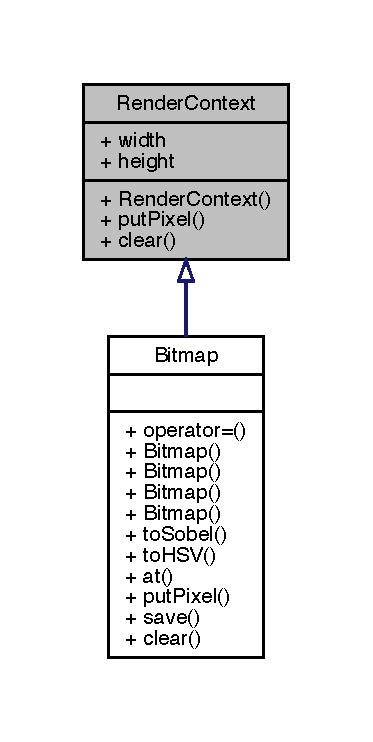
\includegraphics[width=179pt]{class_render_context__inherit__graph}
\end{center}
\end{figure}


Collaboration diagram for Render\+Context\+:\nopagebreak
\begin{figure}[H]
\begin{center}
\leavevmode
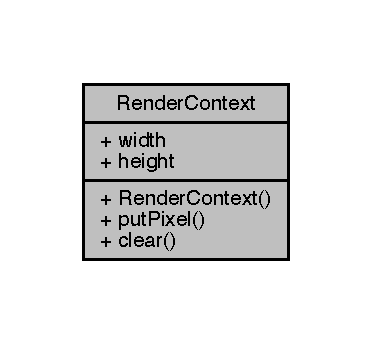
\includegraphics[width=179pt]{class_render_context__coll__graph}
\end{center}
\end{figure}
\subsection*{Public Member Functions}
\begin{DoxyCompactItemize}
\item 
\hyperlink{class_render_context_aff0b414b1aa39e7c5ca4ed5cadf20721}{Render\+Context} (int \hyperlink{class_render_context_a8009663c022d4a60d8a4dbfdb4183f46}{width}, int \hyperlink{class_render_context_a194a36ce3d85ae9ef5b40396e1e2d950}{height})
\item 
virtual void \hyperlink{class_render_context_a722f7e593dc2c480ad5a2a448196c2dc}{put\+Pixel} (int x, int y, glm\+::vec4 color)=0
\item 
virtual void \hyperlink{class_render_context_a9c6a34962ba769bacbb054ea435dfce8}{clear} (glm\+::vec4 color)=0
\end{DoxyCompactItemize}
\subsection*{Public Attributes}
\begin{DoxyCompactItemize}
\item 
int \hyperlink{class_render_context_a8009663c022d4a60d8a4dbfdb4183f46}{width}
\item 
int \hyperlink{class_render_context_a194a36ce3d85ae9ef5b40396e1e2d950}{height}
\end{DoxyCompactItemize}


\subsection{Detailed Description}
Class that is common for every render context. Was useful when i had output to the screen. Tight now only render context is a \hyperlink{class_bitmap}{Bitmap} 

\subsection{Constructor \& Destructor Documentation}
\hypertarget{class_render_context_aff0b414b1aa39e7c5ca4ed5cadf20721}{}\index{Render\+Context@{Render\+Context}!Render\+Context@{Render\+Context}}
\index{Render\+Context@{Render\+Context}!Render\+Context@{Render\+Context}}
\subsubsection[{Render\+Context(int width, int height)}]{\setlength{\rightskip}{0pt plus 5cm}Render\+Context\+::\+Render\+Context (
\begin{DoxyParamCaption}
\item[{int}]{width, }
\item[{int}]{height}
\end{DoxyParamCaption}
)\hspace{0.3cm}{\ttfamily [inline]}}\label{class_render_context_aff0b414b1aa39e7c5ca4ed5cadf20721}
Iniitialize new render context 
\begin{DoxyParams}{Parameters}
{\em width} & new context width \\
\hline
{\em height} & new context height \\
\hline
\end{DoxyParams}


\subsection{Member Function Documentation}
\hypertarget{class_render_context_a9c6a34962ba769bacbb054ea435dfce8}{}\index{Render\+Context@{Render\+Context}!clear@{clear}}
\index{clear@{clear}!Render\+Context@{Render\+Context}}
\subsubsection[{clear(glm\+::vec4 color)=0}]{\setlength{\rightskip}{0pt plus 5cm}virtual void Render\+Context\+::clear (
\begin{DoxyParamCaption}
\item[{glm\+::vec4}]{color}
\end{DoxyParamCaption}
)\hspace{0.3cm}{\ttfamily [pure virtual]}}\label{class_render_context_a9c6a34962ba769bacbb054ea435dfce8}
Abstract method. Fill whole imagwith solid color 
\begin{DoxyParams}{Parameters}
{\em color} & color to use for filling \\
\hline
\end{DoxyParams}


Implemented in \hyperlink{class_bitmap_a409022ea446f41edcce42c076dff1608}{Bitmap}.

\hypertarget{class_render_context_a722f7e593dc2c480ad5a2a448196c2dc}{}\index{Render\+Context@{Render\+Context}!put\+Pixel@{put\+Pixel}}
\index{put\+Pixel@{put\+Pixel}!Render\+Context@{Render\+Context}}
\subsubsection[{put\+Pixel(int x, int y, glm\+::vec4 color)=0}]{\setlength{\rightskip}{0pt plus 5cm}virtual void Render\+Context\+::put\+Pixel (
\begin{DoxyParamCaption}
\item[{int}]{x, }
\item[{int}]{y, }
\item[{glm\+::vec4}]{color}
\end{DoxyParamCaption}
)\hspace{0.3cm}{\ttfamily [pure virtual]}}\label{class_render_context_a722f7e593dc2c480ad5a2a448196c2dc}
Abstract method. Puts pixel of certain color into a render context 
\begin{DoxyParams}[1]{Parameters}
$<$ & {\em name\+::$>$} & $<$\#description\#$>$ \\
\hline
\end{DoxyParams}


Implemented in \hyperlink{class_bitmap_a6f880db00f7d05e6284005a6553aa17c}{Bitmap}.



\subsection{Member Data Documentation}
\hypertarget{class_render_context_a194a36ce3d85ae9ef5b40396e1e2d950}{}\index{Render\+Context@{Render\+Context}!height@{height}}
\index{height@{height}!Render\+Context@{Render\+Context}}
\subsubsection[{height}]{\setlength{\rightskip}{0pt plus 5cm}int Render\+Context\+::height}\label{class_render_context_a194a36ce3d85ae9ef5b40396e1e2d950}
\hypertarget{class_render_context_a8009663c022d4a60d8a4dbfdb4183f46}{}\index{Render\+Context@{Render\+Context}!width@{width}}
\index{width@{width}!Render\+Context@{Render\+Context}}
\subsubsection[{width}]{\setlength{\rightskip}{0pt plus 5cm}int Render\+Context\+::width}\label{class_render_context_a8009663c022d4a60d8a4dbfdb4183f46}


The documentation for this class was generated from the following file\+:\begin{DoxyCompactItemize}
\item 
Texture\+Extractor\+V2/\hyperlink{_render_context_8h}{Render\+Context.\+h}\end{DoxyCompactItemize}

\hypertarget{struct_tex_coord}{}\section{Tex\+Coord Struct Reference}
\label{struct_tex_coord}\index{Tex\+Coord@{Tex\+Coord}}


{\ttfamily \#include $<$Mesh.\+hpp$>$}



Collaboration diagram for Tex\+Coord\+:\nopagebreak
\begin{figure}[H]
\begin{center}
\leavevmode
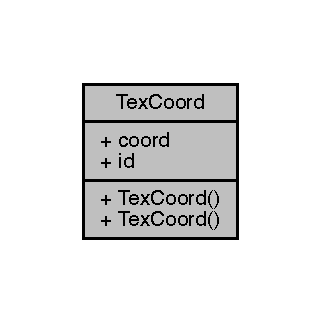
\includegraphics[width=154pt]{struct_tex_coord__coll__graph}
\end{center}
\end{figure}
\subsection*{Public Member Functions}
\begin{DoxyCompactItemize}
\item 
\hyperlink{struct_tex_coord_a02018ed90402d77cb313b581c0ea0561}{Tex\+Coord} (float x, float y)
\item 
\hyperlink{struct_tex_coord_ae1167f68dab931cc523e1f74fa5ad206}{Tex\+Coord} ()
\end{DoxyCompactItemize}
\subsection*{Public Attributes}
\begin{DoxyCompactItemize}
\item 
glm\+::vec2 \hyperlink{struct_tex_coord_a31698d41a1be7a51cbaed632c4fae1e7}{coord}
\item 
uint \hyperlink{struct_tex_coord_aef29d0ef3a3fdcefdda756a2820e2a23}{id}
\end{DoxyCompactItemize}


\subsection{Detailed Description}
Structure that holds texture coordinate 

\subsection{Constructor \& Destructor Documentation}
\hypertarget{struct_tex_coord_a02018ed90402d77cb313b581c0ea0561}{}\index{Tex\+Coord@{Tex\+Coord}!Tex\+Coord@{Tex\+Coord}}
\index{Tex\+Coord@{Tex\+Coord}!Tex\+Coord@{Tex\+Coord}}
\subsubsection[{Tex\+Coord(float x, float y)}]{\setlength{\rightskip}{0pt plus 5cm}Tex\+Coord\+::\+Tex\+Coord (
\begin{DoxyParamCaption}
\item[{float}]{x, }
\item[{float}]{y}
\end{DoxyParamCaption}
)\hspace{0.3cm}{\ttfamily [inline]}}\label{struct_tex_coord_a02018ed90402d77cb313b581c0ea0561}
\hypertarget{struct_tex_coord_ae1167f68dab931cc523e1f74fa5ad206}{}\index{Tex\+Coord@{Tex\+Coord}!Tex\+Coord@{Tex\+Coord}}
\index{Tex\+Coord@{Tex\+Coord}!Tex\+Coord@{Tex\+Coord}}
\subsubsection[{Tex\+Coord()}]{\setlength{\rightskip}{0pt plus 5cm}Tex\+Coord\+::\+Tex\+Coord (
\begin{DoxyParamCaption}
{}
\end{DoxyParamCaption}
)\hspace{0.3cm}{\ttfamily [inline]}}\label{struct_tex_coord_ae1167f68dab931cc523e1f74fa5ad206}


\subsection{Member Data Documentation}
\hypertarget{struct_tex_coord_a31698d41a1be7a51cbaed632c4fae1e7}{}\index{Tex\+Coord@{Tex\+Coord}!coord@{coord}}
\index{coord@{coord}!Tex\+Coord@{Tex\+Coord}}
\subsubsection[{coord}]{\setlength{\rightskip}{0pt plus 5cm}glm\+::vec2 Tex\+Coord\+::coord}\label{struct_tex_coord_a31698d41a1be7a51cbaed632c4fae1e7}
coordinate u and v \hypertarget{struct_tex_coord_aef29d0ef3a3fdcefdda756a2820e2a23}{}\index{Tex\+Coord@{Tex\+Coord}!id@{id}}
\index{id@{id}!Tex\+Coord@{Tex\+Coord}}
\subsubsection[{id}]{\setlength{\rightskip}{0pt plus 5cm}uint Tex\+Coord\+::id}\label{struct_tex_coord_aef29d0ef3a3fdcefdda756a2820e2a23}
coord I\+D 

The documentation for this struct was generated from the following file\+:\begin{DoxyCompactItemize}
\item 
Texture\+Extractor\+V2/\hyperlink{_mesh_8hpp}{Mesh.\+hpp}\end{DoxyCompactItemize}

\hypertarget{class_texture_edge}{}\section{Texture\+Edge Class Reference}
\label{class_texture_edge}\index{Texture\+Edge@{Texture\+Edge}}
\subsection*{Public Member Functions}
\begin{DoxyCompactItemize}
\item 
\hypertarget{class_texture_edge_adbdc3b619799de6ef2ca4a60b072a7f7}{}{\bfseries Texture\+Edge} (\hyperlink{struct_vertex}{Vertex} start, \hyperlink{struct_vertex}{Vertex} end, \hyperlink{class_texture_gradient}{Texture\+Gradient} gradient, int min\+Y\+Vert\+Index)\label{class_texture_edge_adbdc3b619799de6ef2ca4a60b072a7f7}

\item 
\hypertarget{class_texture_edge_a15f585808723671c895a71792fe19c60}{}{\bfseries Texture\+Edge} (\hyperlink{struct_vertex}{Vertex} start, \hyperlink{struct_vertex}{Vertex} end)\label{class_texture_edge_a15f585808723671c895a71792fe19c60}

\item 
\hypertarget{class_texture_edge_a65e70bfe49405d2bd92b32066fdc0752}{}void {\bfseries Step} ()\label{class_texture_edge_a65e70bfe49405d2bd92b32066fdc0752}

\end{DoxyCompactItemize}
\subsection*{Public Attributes}
\begin{DoxyCompactItemize}
\item 
\hypertarget{class_texture_edge_a7c3b80e498b2695a022e27c9585ce179}{}float {\bfseries current\+X}\label{class_texture_edge_a7c3b80e498b2695a022e27c9585ce179}

\item 
\hypertarget{class_texture_edge_a25cef82338114b36eb787cf7388f51c2}{}float {\bfseries x\+Step}\label{class_texture_edge_a25cef82338114b36eb787cf7388f51c2}

\item 
\hypertarget{class_texture_edge_aedbd23f82d3d7bcefa909a817ecd1352}{}float {\bfseries y\+Start}\label{class_texture_edge_aedbd23f82d3d7bcefa909a817ecd1352}

\item 
\hypertarget{class_texture_edge_a2974871a249726ee903849f14ded2bf5}{}float {\bfseries y\+End}\label{class_texture_edge_a2974871a249726ee903849f14ded2bf5}

\item 
\hypertarget{class_texture_edge_a6dd2c8650dd32b7150b3f6b62b338360}{}float {\bfseries one\+Over\+Z}\label{class_texture_edge_a6dd2c8650dd32b7150b3f6b62b338360}

\item 
\hypertarget{class_texture_edge_a074ed9078d97be9319aa786ffdcf5a2e}{}float {\bfseries one\+Over\+Z\+Step}\label{class_texture_edge_a074ed9078d97be9319aa786ffdcf5a2e}

\item 
\hypertarget{class_texture_edge_abb286c00988b8204557806352f3a08fb}{}glm\+::vec2 {\bfseries photo\+Coord}\label{class_texture_edge_abb286c00988b8204557806352f3a08fb}

\item 
\hypertarget{class_texture_edge_abe3b2ba9ef56a213949cfd899b0bcd86}{}glm\+::vec2 {\bfseries photo\+Coord\+Step}\label{class_texture_edge_abe3b2ba9ef56a213949cfd899b0bcd86}

\item 
\hypertarget{class_texture_edge_ab0f8a2b476e5a4bc28f7d95b0753ac69}{}glm\+::vec4 {\bfseries color}\label{class_texture_edge_ab0f8a2b476e5a4bc28f7d95b0753ac69}

\item 
\hypertarget{class_texture_edge_a978d737a720ca72aac38a02e6d190c05}{}glm\+::vec4 {\bfseries color\+Step}\label{class_texture_edge_a978d737a720ca72aac38a02e6d190c05}

\end{DoxyCompactItemize}


The documentation for this class was generated from the following files\+:\begin{DoxyCompactItemize}
\item 
Texture\+Extractor\+V2/Texture\+Edge.\+hpp\item 
Texture\+Extractor\+V2/Texture\+Edge.\+cpp\end{DoxyCompactItemize}

\hypertarget{class_texture_extractor}{}\section{Texture\+Extractor Class Reference}
\label{class_texture_extractor}\index{Texture\+Extractor@{Texture\+Extractor}}


{\ttfamily \#include $<$Texture\+Extractor.\+hpp$>$}

\subsection*{Public Member Functions}
\begin{DoxyCompactItemize}
\item 
bool \hyperlink{class_texture_extractor_a5d1efa1c5208f8a1e67142dd38fbf5a2}{prepare\+Views} ()
\item 
bool \hyperlink{class_texture_extractor_af7e364344bda2e0c6784c82b50a6f979}{calculate\+Data\+Costs} ()
\item 
bool \hyperlink{class_texture_extractor_abeb85c1ced22591fda614af1f351e817}{select\+Views} ()
\item 
void \hyperlink{class_texture_extractor_ae02d3f7a8ebf636fd7fc17ab13570f59}{set\+Mesh} (const \hyperlink{class_mesh}{Mesh} \&m)
\item 
bool \hyperlink{class_texture_extractor_a58176e3b3dc4f2edaaa900a7e922ab05}{generate\+Texture} ()
\item 
bool \hyperlink{class_texture_extractor_aeda3235d55d4dec0d1f40d42bc97a2c4}{generate\+Texture\+For\+Object} (\hyperlink{struct_object}{Object} \&object)
\item 
uint \hyperlink{class_texture_extractor_a57b2eef07397ceeedf461343aff6afbc}{number\+Of\+Views} ()
\item 
bool \hyperlink{class_texture_extractor_ad3855ac7764dc5af24e776e928bed802}{read\+Labels\+From\+File} ()
\item 
bool \hyperlink{class_texture_extractor_a9f3605a51c466cca05f8ff216c84d574}{read\+Data\+Costs\+From\+File} ()
\item 
void \hyperlink{class_texture_extractor_a196dde057ce49bcae8cc7d07cf00f8cc}{postprocess\+Data\+Costs} ()
\item 
void \hyperlink{class_texture_extractor_a82baa1e8ae7c17bd9f1d44b431f82f86}{check\+Camera\+Info} ()
\item 
void \hyperlink{class_texture_extractor_a93b91c57ec384eaf45a36c917b6c9e63}{check\+Camera\+Info} (uint view\+Id)
\item 
void \hyperlink{class_texture_extractor_a77c9ce096ece162dac08599fc7c0ee47}{render\+View} (\hyperlink{class_bitmap}{Bitmap} \&bitmap, uint view\+Id)
\item 
void \hyperlink{class_texture_extractor_ab805f165c443e6f1616ee0be9afa74e3}{render\+View\+And\+Depth} (\hyperlink{class_bitmap}{Bitmap} \&bitmap, \hyperlink{class_bitmap}{Bitmap} \&bitmap\+Depth, uint view\+Id)
\end{DoxyCompactItemize}


\subsection{Detailed Description}
Main class. Manages general extraction tasks 

\subsection{Member Function Documentation}
\hypertarget{class_texture_extractor_af7e364344bda2e0c6784c82b50a6f979}{}\index{Texture\+Extractor@{Texture\+Extractor}!calculate\+Data\+Costs@{calculate\+Data\+Costs}}
\index{calculate\+Data\+Costs@{calculate\+Data\+Costs}!Texture\+Extractor@{Texture\+Extractor}}
\subsubsection[{calculate\+Data\+Costs()}]{\setlength{\rightskip}{0pt plus 5cm}bool Texture\+Extractor\+::calculate\+Data\+Costs (
\begin{DoxyParamCaption}
{}
\end{DoxyParamCaption}
)}\label{class_texture_extractor_af7e364344bda2e0c6784c82b50a6f979}
Starts datacost calcualtation. \hypertarget{class_texture_extractor_a82baa1e8ae7c17bd9f1d44b431f82f86}{}\index{Texture\+Extractor@{Texture\+Extractor}!check\+Camera\+Info@{check\+Camera\+Info}}
\index{check\+Camera\+Info@{check\+Camera\+Info}!Texture\+Extractor@{Texture\+Extractor}}
\subsubsection[{check\+Camera\+Info()}]{\setlength{\rightskip}{0pt plus 5cm}void Texture\+Extractor\+::check\+Camera\+Info (
\begin{DoxyParamCaption}
{}
\end{DoxyParamCaption}
)}\label{class_texture_extractor_a82baa1e8ae7c17bd9f1d44b431f82f86}
D\+E\+B\+U\+G\+: prints out camera info \hypertarget{class_texture_extractor_a93b91c57ec384eaf45a36c917b6c9e63}{}\index{Texture\+Extractor@{Texture\+Extractor}!check\+Camera\+Info@{check\+Camera\+Info}}
\index{check\+Camera\+Info@{check\+Camera\+Info}!Texture\+Extractor@{Texture\+Extractor}}
\subsubsection[{check\+Camera\+Info(uint view\+Id)}]{\setlength{\rightskip}{0pt plus 5cm}void Texture\+Extractor\+::check\+Camera\+Info (
\begin{DoxyParamCaption}
\item[{uint}]{view\+Id}
\end{DoxyParamCaption}
)}\label{class_texture_extractor_a93b91c57ec384eaf45a36c917b6c9e63}
D\+E\+B\+U\+G\+: prints out camera info for one camera only \hypertarget{class_texture_extractor_a58176e3b3dc4f2edaaa900a7e922ab05}{}\index{Texture\+Extractor@{Texture\+Extractor}!generate\+Texture@{generate\+Texture}}
\index{generate\+Texture@{generate\+Texture}!Texture\+Extractor@{Texture\+Extractor}}
\subsubsection[{generate\+Texture()}]{\setlength{\rightskip}{0pt plus 5cm}bool Texture\+Extractor\+::generate\+Texture (
\begin{DoxyParamCaption}
{}
\end{DoxyParamCaption}
)}\label{class_texture_extractor_a58176e3b3dc4f2edaaa900a7e922ab05}
Using labeling starts to generate texture files for all the objects in the mesh \hypertarget{class_texture_extractor_aeda3235d55d4dec0d1f40d42bc97a2c4}{}\index{Texture\+Extractor@{Texture\+Extractor}!generate\+Texture\+For\+Object@{generate\+Texture\+For\+Object}}
\index{generate\+Texture\+For\+Object@{generate\+Texture\+For\+Object}!Texture\+Extractor@{Texture\+Extractor}}
\subsubsection[{generate\+Texture\+For\+Object(\+Object \&object)}]{\setlength{\rightskip}{0pt plus 5cm}bool Texture\+Extractor\+::generate\+Texture\+For\+Object (
\begin{DoxyParamCaption}
\item[{{\bf Object} \&}]{object}
\end{DoxyParamCaption}
)}\label{class_texture_extractor_aeda3235d55d4dec0d1f40d42bc97a2c4}
Generates textures for a single object 
\begin{DoxyParams}{Parameters}
{\em object} & target object \\
\hline
\end{DoxyParams}
\hypertarget{class_texture_extractor_a57b2eef07397ceeedf461343aff6afbc}{}\index{Texture\+Extractor@{Texture\+Extractor}!number\+Of\+Views@{number\+Of\+Views}}
\index{number\+Of\+Views@{number\+Of\+Views}!Texture\+Extractor@{Texture\+Extractor}}
\subsubsection[{number\+Of\+Views()}]{\setlength{\rightskip}{0pt plus 5cm}uint Texture\+Extractor\+::number\+Of\+Views (
\begin{DoxyParamCaption}
{}
\end{DoxyParamCaption}
)\hspace{0.3cm}{\ttfamily [inline]}}\label{class_texture_extractor_a57b2eef07397ceeedf461343aff6afbc}
returns a number of views(source photographs) \hypertarget{class_texture_extractor_a196dde057ce49bcae8cc7d07cf00f8cc}{}\index{Texture\+Extractor@{Texture\+Extractor}!postprocess\+Data\+Costs@{postprocess\+Data\+Costs}}
\index{postprocess\+Data\+Costs@{postprocess\+Data\+Costs}!Texture\+Extractor@{Texture\+Extractor}}
\subsubsection[{postprocess\+Data\+Costs()}]{\setlength{\rightskip}{0pt plus 5cm}void Texture\+Extractor\+::postprocess\+Data\+Costs (
\begin{DoxyParamCaption}
{}
\end{DoxyParamCaption}
)}\label{class_texture_extractor_a196dde057ce49bcae8cc7d07cf00f8cc}
Uses patch qulity to calculate datacosts and does color consistency check \hypertarget{class_texture_extractor_a5d1efa1c5208f8a1e67142dd38fbf5a2}{}\index{Texture\+Extractor@{Texture\+Extractor}!prepare\+Views@{prepare\+Views}}
\index{prepare\+Views@{prepare\+Views}!Texture\+Extractor@{Texture\+Extractor}}
\subsubsection[{prepare\+Views()}]{\setlength{\rightskip}{0pt plus 5cm}bool Texture\+Extractor\+::prepare\+Views (
\begin{DoxyParamCaption}
{}
\end{DoxyParamCaption}
)}\label{class_texture_extractor_a5d1efa1c5208f8a1e67142dd38fbf5a2}
Reads and prepares views using the bundler file and camera list. Calculates all the nessecary matricies and parametrs \hypertarget{class_texture_extractor_a9f3605a51c466cca05f8ff216c84d574}{}\index{Texture\+Extractor@{Texture\+Extractor}!read\+Data\+Costs\+From\+File@{read\+Data\+Costs\+From\+File}}
\index{read\+Data\+Costs\+From\+File@{read\+Data\+Costs\+From\+File}!Texture\+Extractor@{Texture\+Extractor}}
\subsubsection[{read\+Data\+Costs\+From\+File()}]{\setlength{\rightskip}{0pt plus 5cm}bool Texture\+Extractor\+::read\+Data\+Costs\+From\+File (
\begin{DoxyParamCaption}
{}
\end{DoxyParamCaption}
)}\label{class_texture_extractor_a9f3605a51c466cca05f8ff216c84d574}
Reads and verifies precomputed labeling from file. \hypertarget{class_texture_extractor_ad3855ac7764dc5af24e776e928bed802}{}\index{Texture\+Extractor@{Texture\+Extractor}!read\+Labels\+From\+File@{read\+Labels\+From\+File}}
\index{read\+Labels\+From\+File@{read\+Labels\+From\+File}!Texture\+Extractor@{Texture\+Extractor}}
\subsubsection[{read\+Labels\+From\+File()}]{\setlength{\rightskip}{0pt plus 5cm}bool Texture\+Extractor\+::read\+Labels\+From\+File (
\begin{DoxyParamCaption}
{}
\end{DoxyParamCaption}
)}\label{class_texture_extractor_ad3855ac7764dc5af24e776e928bed802}
Reads and verifies precomputed labeling from file. \hypertarget{class_texture_extractor_a77c9ce096ece162dac08599fc7c0ee47}{}\index{Texture\+Extractor@{Texture\+Extractor}!render\+View@{render\+View}}
\index{render\+View@{render\+View}!Texture\+Extractor@{Texture\+Extractor}}
\subsubsection[{render\+View(\+Bitmap \&bitmap, uint view\+Id)}]{\setlength{\rightskip}{0pt plus 5cm}void Texture\+Extractor\+::render\+View (
\begin{DoxyParamCaption}
\item[{{\bf Bitmap} \&}]{bitmap, }
\item[{uint}]{view\+Id}
\end{DoxyParamCaption}
)}\label{class_texture_extractor_a77c9ce096ece162dac08599fc7c0ee47}
D\+E\+B\+U\+G\+: renders a view 
\begin{DoxyParams}{Parameters}
{\em bitmap} & image target. \\
\hline
{\em view\+I\+D} & view to replicate \\
\hline
\end{DoxyParams}
\hypertarget{class_texture_extractor_ab805f165c443e6f1616ee0be9afa74e3}{}\index{Texture\+Extractor@{Texture\+Extractor}!render\+View\+And\+Depth@{render\+View\+And\+Depth}}
\index{render\+View\+And\+Depth@{render\+View\+And\+Depth}!Texture\+Extractor@{Texture\+Extractor}}
\subsubsection[{render\+View\+And\+Depth(\+Bitmap \&bitmap, Bitmap \&bitmap\+Depth, uint view\+Id)}]{\setlength{\rightskip}{0pt plus 5cm}void Texture\+Extractor\+::render\+View\+And\+Depth (
\begin{DoxyParamCaption}
\item[{{\bf Bitmap} \&}]{bitmap, }
\item[{{\bf Bitmap} \&}]{bitmap\+Depth, }
\item[{uint}]{view\+Id}
\end{DoxyParamCaption}
)}\label{class_texture_extractor_ab805f165c443e6f1616ee0be9afa74e3}
D\+E\+B\+U\+G\+: renders a view and depth map 
\begin{DoxyParams}{Parameters}
{\em bitmap} & output image target. \\
\hline
{\em bitmap\+Depth} & output depth image target. \\
\hline
{\em view\+I\+D} & view to replicate \\
\hline
\end{DoxyParams}
\hypertarget{class_texture_extractor_abeb85c1ced22591fda614af1f351e817}{}\index{Texture\+Extractor@{Texture\+Extractor}!select\+Views@{select\+Views}}
\index{select\+Views@{select\+Views}!Texture\+Extractor@{Texture\+Extractor}}
\subsubsection[{select\+Views()}]{\setlength{\rightskip}{0pt plus 5cm}bool Texture\+Extractor\+::select\+Views (
\begin{DoxyParamCaption}
{}
\end{DoxyParamCaption}
)}\label{class_texture_extractor_abeb85c1ced22591fda614af1f351e817}
Starts a labeling process \hypertarget{class_texture_extractor_ae02d3f7a8ebf636fd7fc17ab13570f59}{}\index{Texture\+Extractor@{Texture\+Extractor}!set\+Mesh@{set\+Mesh}}
\index{set\+Mesh@{set\+Mesh}!Texture\+Extractor@{Texture\+Extractor}}
\subsubsection[{set\+Mesh(const Mesh \&m)}]{\setlength{\rightskip}{0pt plus 5cm}void Texture\+Extractor\+::set\+Mesh (
\begin{DoxyParamCaption}
\item[{const {\bf Mesh} \&}]{m}
\end{DoxyParamCaption}
)\hspace{0.3cm}{\ttfamily [inline]}}\label{class_texture_extractor_ae02d3f7a8ebf636fd7fc17ab13570f59}
sets a working mesh 
\begin{DoxyParams}{Parameters}
{\em M} & input mesh \\
\hline
\end{DoxyParams}


The documentation for this class was generated from the following files\+:\begin{DoxyCompactItemize}
\item 
Texture\+Extractor\+V2/Texture\+Extractor.\+hpp\item 
Texture\+Extractor\+V2/Texture\+Extractor.\+cpp\item 
Texture\+Extractor\+V2/Texture\+Extractor\+\_\+map\+Map.\+cpp\end{DoxyCompactItemize}

\hypertarget{class_texture_gradient}{}\section{Texture\+Gradient Class Reference}
\label{class_texture_gradient}\index{Texture\+Gradient@{Texture\+Gradient}}
\subsection*{Public Member Functions}
\begin{DoxyCompactItemize}
\item 
\hypertarget{class_texture_gradient_ac52b7944976524744bcc35ec9918b09c}{}{\bfseries Texture\+Gradient} (\hyperlink{struct_vertex}{Vertex} min\+Y\+Vert, \hyperlink{struct_vertex}{Vertex} mid\+Y\+Vert, \hyperlink{struct_vertex}{Vertex} max\+Y\+Vert)\label{class_texture_gradient_ac52b7944976524744bcc35ec9918b09c}

\item 
\hypertarget{class_texture_gradient_a1aac43bd7935b57410122be0affa0896}{}{\bfseries Texture\+Gradient} (\hyperlink{struct_vertex}{Vertex} min\+Y\+Vert, \hyperlink{struct_vertex}{Vertex} mid\+Y\+Vert, \hyperlink{struct_vertex}{Vertex} max\+Y\+Vert, glm\+::vec4 color\mbox{[}3\mbox{]})\label{class_texture_gradient_a1aac43bd7935b57410122be0affa0896}

\end{DoxyCompactItemize}
\subsection*{Public Attributes}
\begin{DoxyCompactItemize}
\item 
\hypertarget{class_texture_gradient_a34bee5b4f0894efeec794704d3fd2cec}{}float {\bfseries photo\+Coord\+X\+X\+Step}\label{class_texture_gradient_a34bee5b4f0894efeec794704d3fd2cec}

\item 
\hypertarget{class_texture_gradient_ad667fab8a0c76c19fdb5d27510b5a9ba}{}float {\bfseries photo\+Coord\+X\+Y\+Step}\label{class_texture_gradient_ad667fab8a0c76c19fdb5d27510b5a9ba}

\item 
\hypertarget{class_texture_gradient_af13ceccfc1629d08233d025c1d060992}{}float {\bfseries photo\+Coord\+Y\+X\+Step}\label{class_texture_gradient_af13ceccfc1629d08233d025c1d060992}

\item 
\hypertarget{class_texture_gradient_a12b19a4e9245a4c71f9bb1c36f40f94d}{}float {\bfseries photo\+Coord\+Y\+Y\+Step}\label{class_texture_gradient_a12b19a4e9245a4c71f9bb1c36f40f94d}

\item 
\hypertarget{class_texture_gradient_a504ba2546491bbe0eb80c9e496020aff}{}glm\+::vec2 {\bfseries one\+Over\+Z\+Step}\label{class_texture_gradient_a504ba2546491bbe0eb80c9e496020aff}

\item 
\hypertarget{class_texture_gradient_a864076b3aeea93295c0f3d262ede9fac}{}glm\+::vec4 {\bfseries photo\+Coords} \mbox{[}3\mbox{]}\label{class_texture_gradient_a864076b3aeea93295c0f3d262ede9fac}

\item 
\hypertarget{class_texture_gradient_ac3a61d0f068bf9e1716d4a6043fb39c3}{}glm\+::vec4 {\bfseries color\+X\+Step}\label{class_texture_gradient_ac3a61d0f068bf9e1716d4a6043fb39c3}

\item 
\hypertarget{class_texture_gradient_ac34b317ff76b5493b159b3491df26839}{}glm\+::vec4 {\bfseries color\+Y\+Step}\label{class_texture_gradient_ac34b317ff76b5493b159b3491df26839}

\item 
\hypertarget{class_texture_gradient_aad5614bae7a7361a1b82b69d9b082ea6}{}glm\+::vec4 {\bfseries color} \mbox{[}3\mbox{]}\label{class_texture_gradient_aad5614bae7a7361a1b82b69d9b082ea6}

\item 
\hypertarget{class_texture_gradient_af7d99a3ca4515f65a8afeb5139cd2d8e}{}float {\bfseries one\+Over\+Z} \mbox{[}3\mbox{]}\label{class_texture_gradient_af7d99a3ca4515f65a8afeb5139cd2d8e}

\end{DoxyCompactItemize}


The documentation for this class was generated from the following files\+:\begin{DoxyCompactItemize}
\item 
Texture\+Extractor\+V2/Texture\+Gradient.\+hpp\item 
Texture\+Extractor\+V2/Texture\+Gradient.\+cpp\end{DoxyCompactItemize}

\hypertarget{struct_texture_patch}{}\section{Texture\+Patch Struct Reference}
\label{struct_texture_patch}\index{Texture\+Patch@{Texture\+Patch}}


{\ttfamily \#include $<$Texture\+Patch.\+hpp$>$}

\subsection*{Public Attributes}
\begin{DoxyCompactItemize}
\item 
std\+::set$<$ uint $>$ \hyperlink{struct_texture_patch_a6508eab52b765ffa3f5b185956334f47}{my\+Triangles}
\item 
std\+::vector$<$ \hyperlink{struct_edge_vertex}{Edge\+Vertex} $>$ \hyperlink{struct_texture_patch_a93366f5b9cc0d02ba08ffb4fba64d977}{edge\+Verticies}
\item 
std\+::set$<$ uint $>$ \hyperlink{struct_texture_patch_a002b3455ab2599b42b78c34c1d887f94}{neighbour\+Triangles}
\item 
uint \hyperlink{struct_texture_patch_a359bb72c7d9793ff22e9d6272b016521}{patch\+I\+D}
\item 
uint \hyperlink{struct_texture_patch_a97acb0ad9531af6cc0c366640d3575e1}{view\+I\+D}
\item 
glm\+::vec4 \hyperlink{struct_texture_patch_a1285c94f40ae56464f33eaf69fb93617}{mean\+Color\+Diff}
\end{DoxyCompactItemize}


\subsection{Detailed Description}
Sructure that defines texture patch set. All all the adjacent texture polyogns that are assigned the same labeling 

\subsection{Member Data Documentation}
\hypertarget{struct_texture_patch_a93366f5b9cc0d02ba08ffb4fba64d977}{}\index{Texture\+Patch@{Texture\+Patch}!edge\+Verticies@{edge\+Verticies}}
\index{edge\+Verticies@{edge\+Verticies}!Texture\+Patch@{Texture\+Patch}}
\subsubsection[{edge\+Verticies}]{\setlength{\rightskip}{0pt plus 5cm}std\+::vector$<${\bf Edge\+Vertex}$>$ Texture\+Patch\+::edge\+Verticies}\label{struct_texture_patch_a93366f5b9cc0d02ba08ffb4fba64d977}
set of vertex samples on the edge of the set \hypertarget{struct_texture_patch_a1285c94f40ae56464f33eaf69fb93617}{}\index{Texture\+Patch@{Texture\+Patch}!mean\+Color\+Diff@{mean\+Color\+Diff}}
\index{mean\+Color\+Diff@{mean\+Color\+Diff}!Texture\+Patch@{Texture\+Patch}}
\subsubsection[{mean\+Color\+Diff}]{\setlength{\rightskip}{0pt plus 5cm}glm\+::vec4 Texture\+Patch\+::mean\+Color\+Diff}\label{struct_texture_patch_a1285c94f40ae56464f33eaf69fb93617}
Mean color differene calculated using edge samples \hypertarget{struct_texture_patch_a6508eab52b765ffa3f5b185956334f47}{}\index{Texture\+Patch@{Texture\+Patch}!my\+Triangles@{my\+Triangles}}
\index{my\+Triangles@{my\+Triangles}!Texture\+Patch@{Texture\+Patch}}
\subsubsection[{my\+Triangles}]{\setlength{\rightskip}{0pt plus 5cm}std\+::set$<$uint$>$ Texture\+Patch\+::my\+Triangles}\label{struct_texture_patch_a6508eab52b765ffa3f5b185956334f47}
set of triangle ids that belong to a set \hypertarget{struct_texture_patch_a002b3455ab2599b42b78c34c1d887f94}{}\index{Texture\+Patch@{Texture\+Patch}!neighbour\+Triangles@{neighbour\+Triangles}}
\index{neighbour\+Triangles@{neighbour\+Triangles}!Texture\+Patch@{Texture\+Patch}}
\subsubsection[{neighbour\+Triangles}]{\setlength{\rightskip}{0pt plus 5cm}std\+::set$<$uint$>$ Texture\+Patch\+::neighbour\+Triangles}\label{struct_texture_patch_a002b3455ab2599b42b78c34c1d887f94}
set of neighbouring triangles that are adjacent to our set but are assigned a different source image \hypertarget{struct_texture_patch_a359bb72c7d9793ff22e9d6272b016521}{}\index{Texture\+Patch@{Texture\+Patch}!patch\+I\+D@{patch\+I\+D}}
\index{patch\+I\+D@{patch\+I\+D}!Texture\+Patch@{Texture\+Patch}}
\subsubsection[{patch\+I\+D}]{\setlength{\rightskip}{0pt plus 5cm}uint Texture\+Patch\+::patch\+I\+D}\label{struct_texture_patch_a359bb72c7d9793ff22e9d6272b016521}
I\+D of a patch set \hypertarget{struct_texture_patch_a97acb0ad9531af6cc0c366640d3575e1}{}\index{Texture\+Patch@{Texture\+Patch}!view\+I\+D@{view\+I\+D}}
\index{view\+I\+D@{view\+I\+D}!Texture\+Patch@{Texture\+Patch}}
\subsubsection[{view\+I\+D}]{\setlength{\rightskip}{0pt plus 5cm}uint Texture\+Patch\+::view\+I\+D}\label{struct_texture_patch_a97acb0ad9531af6cc0c366640d3575e1}
I\+D of a view assignment common to a set 

The documentation for this struct was generated from the following file\+:\begin{DoxyCompactItemize}
\item 
Texture\+Extractor\+V2/Texture\+Patch.\+hpp\end{DoxyCompactItemize}

\hypertarget{struct_texture_patch_dictionary}{}\section{Texture\+Patch\+Dictionary Struct Reference}
\label{struct_texture_patch_dictionary}\index{Texture\+Patch\+Dictionary@{Texture\+Patch\+Dictionary}}
\subsection*{Public Member Functions}
\begin{DoxyCompactItemize}
\item 
\hypertarget{struct_texture_patch_dictionary_aba62d1d0383da168f7bdef1050970a92}{}uint {\bfseries gen\+New\+Patch} ()\label{struct_texture_patch_dictionary_aba62d1d0383da168f7bdef1050970a92}

\end{DoxyCompactItemize}
\subsection*{Public Attributes}
\begin{DoxyCompactItemize}
\item 
\hypertarget{struct_texture_patch_dictionary_a188d2b68586a902ef8c969458e9001c6}{}std\+::map$<$ uint, uint $>$ {\bfseries triangle\+Membership}\label{struct_texture_patch_dictionary_a188d2b68586a902ef8c969458e9001c6}

\item 
\hypertarget{struct_texture_patch_dictionary_a21c6633d4831bd84be792b45020f3805}{}std\+::map$<$ uint, \hyperlink{struct_texture_patch}{Texture\+Patch} $>$ {\bfseries patches}\label{struct_texture_patch_dictionary_a21c6633d4831bd84be792b45020f3805}

\end{DoxyCompactItemize}


The documentation for this struct was generated from the following file\+:\begin{DoxyCompactItemize}
\item 
Texture\+Extractor\+V2/Texture\+Patch.\+hpp\end{DoxyCompactItemize}

\hypertarget{class_timer}{}\section{Timer Class Reference}
\label{class_timer}\index{Timer@{Timer}}
\subsection*{Public Member Functions}
\begin{DoxyCompactItemize}
\item 
\hypertarget{class_timer_a3a8b5272198d029779dc9302a54305a8}{}void {\bfseries start} ()\label{class_timer_a3a8b5272198d029779dc9302a54305a8}

\item 
\hypertarget{class_timer_aa7dd6187a7dec39be17dfb4f6184db16}{}std\+::string {\bfseries stop\+Get\+Results} ()\label{class_timer_aa7dd6187a7dec39be17dfb4f6184db16}

\item 
\hypertarget{class_timer_a573a098aacebc4be22ce73bd42725e17}{}std\+::string {\bfseries stop\+Get\+Results} (const std\+::string \&message\+Prefix)\label{class_timer_a573a098aacebc4be22ce73bd42725e17}

\end{DoxyCompactItemize}


The documentation for this class was generated from the following files\+:\begin{DoxyCompactItemize}
\item 
Texture\+Extractor\+V2/Timer.\+hpp\item 
Texture\+Extractor\+V2/Timer.\+cpp\end{DoxyCompactItemize}

\hypertarget{class_transformation}{}\section{Transformation Class Reference}
\label{class_transformation}\index{Transformation@{Transformation}}
\subsection*{Public Member Functions}
\begin{DoxyCompactItemize}
\item 
\hypertarget{class_transformation_a9e066efd2a4d28a13d1bdb54de254bec}{}{\bfseries Transformation} (const glm\+::vec3 \&pos=glm\+::vec3(), const glm\+::vec3 \&rot=glm\+::vec3(), const glm\+::vec3 \&scale=glm\+::vec3(1.\+0, 1.\+0, 1.\+0))\label{class_transformation_a9e066efd2a4d28a13d1bdb54de254bec}

\item 
\hypertarget{class_transformation_aba67dba23c6180e047f8172c461a7554}{}void {\bfseries set\+Aspect\+Ratio} (int width, int height)\label{class_transformation_aba67dba23c6180e047f8172c461a7554}

\item 
\hypertarget{class_transformation_a93295202dbfbb2b450d5bd893ee3237b}{}void {\bfseries set\+Camera} (const \hyperlink{class_camera}{Camera} \&camera)\label{class_transformation_a93295202dbfbb2b450d5bd893ee3237b}

\item 
\hypertarget{class_transformation_ae2dcb616a0231a331ed97a9ef5704849}{}void {\bfseries set\+Screen\+Transform} (int half\+Height, int half\+Width)\label{class_transformation_ae2dcb616a0231a331ed97a9ef5704849}

\item 
\hypertarget{class_transformation_a9bb89f79245297795c78f62ca6b29efd}{}\hyperlink{struct_vertex}{Vertex} {\bfseries do\+Perspective\+Devide} (const \hyperlink{struct_vertex}{Vertex} \&coord) const \label{class_transformation_a9bb89f79245297795c78f62ca6b29efd}

\item 
\hypertarget{class_transformation_a0a6033abab9c32b487c90b95fd1a2df3}{}glm\+::mat4 {\bfseries get\+Model\+Matrix} () const \label{class_transformation_a0a6033abab9c32b487c90b95fd1a2df3}

\item 
\hypertarget{class_transformation_a4d2b0cd9862c2b0485740a896617c867}{}glm\+::mat4 {\bfseries get\+Screen\+Transform} () const \label{class_transformation_a4d2b0cd9862c2b0485740a896617c867}

\item 
\hypertarget{class_transformation_a5f57370067951aecad8b40bec887c2ef}{}glm\+::mat4 {\bfseries get\+View\+Projection} () const \label{class_transformation_a5f57370067951aecad8b40bec887c2ef}

\end{DoxyCompactItemize}
\subsection*{Public Attributes}
\begin{DoxyCompactItemize}
\item 
\hypertarget{class_transformation_aeaf15f9849ac1a0dc2b5f7a7da12e0ed}{}glm\+::vec3 {\bfseries pos}\label{class_transformation_aeaf15f9849ac1a0dc2b5f7a7da12e0ed}

\item 
\hypertarget{class_transformation_a4d41188f5f002453bb288c32452c79d2}{}glm\+::vec3 {\bfseries rot}\label{class_transformation_a4d41188f5f002453bb288c32452c79d2}

\item 
\hypertarget{class_transformation_abaca94f82d6d4c1515c133e638624724}{}glm\+::vec3 {\bfseries scale}\label{class_transformation_abaca94f82d6d4c1515c133e638624724}

\end{DoxyCompactItemize}


The documentation for this class was generated from the following files\+:\begin{DoxyCompactItemize}
\item 
Texture\+Extractor\+V2/Transformation.\+hpp\item 
Texture\+Extractor\+V2/Transformation.\+cpp\end{DoxyCompactItemize}

\hypertarget{struct_triangle}{}\section{Triangle Struct Reference}
\label{struct_triangle}\index{Triangle@{Triangle}}
\subsection*{Public Member Functions}
\begin{DoxyCompactItemize}
\item 
\hypertarget{struct_triangle_a88209808e641989a51c9f5e23b8857f5}{}{\bfseries Triangle} (const uint verticies\mbox{[}3\mbox{]})\label{struct_triangle_a88209808e641989a51c9f5e23b8857f5}

\end{DoxyCompactItemize}
\subsection*{Public Attributes}
\begin{DoxyCompactItemize}
\item 
\hypertarget{struct_triangle_ae6371f947daaa0debff04c10b6fadf74}{}uint {\bfseries verticies} \mbox{[}3\mbox{]}\label{struct_triangle_ae6371f947daaa0debff04c10b6fadf74}

\item 
\hypertarget{struct_triangle_a2d3dc46484a1d1cc2802caaaa4a5f1cf}{}std\+::map$<$ uint, uint $>$ {\bfseries tex\+Coords}\label{struct_triangle_a2d3dc46484a1d1cc2802caaaa4a5f1cf}

\item 
\hypertarget{struct_triangle_a9e82ef210ec3746af058c3b4793bd34d}{}std\+::map$<$ uint, uint $>$ {\bfseries normal\+Vecs}\label{struct_triangle_a9e82ef210ec3746af058c3b4793bd34d}

\item 
\hypertarget{struct_triangle_a2b02bfd83feba5fe297836b900a62c92}{}uint {\bfseries id}\label{struct_triangle_a2b02bfd83feba5fe297836b900a62c92}

\item 
\hypertarget{struct_triangle_a18682ece909b0d90107ac391f37f5cd4}{}uint {\bfseries view\+Id} = 0\label{struct_triangle_a18682ece909b0d90107ac391f37f5cd4}

\item 
\hypertarget{struct_triangle_a980bbf270a13c5ac9112e6e8c8c2ea89}{}\hyperlink{struct_bounding_box}{Bounding\+Box} {\bfseries bounding\+Box}\label{struct_triangle_a980bbf270a13c5ac9112e6e8c8c2ea89}

\end{DoxyCompactItemize}


The documentation for this struct was generated from the following file\+:\begin{DoxyCompactItemize}
\item 
Texture\+Extractor\+V2/Mesh.\+hpp\end{DoxyCompactItemize}

\hypertarget{struct_vertex}{}\section{Vertex Struct Reference}
\label{struct_vertex}\index{Vertex@{Vertex}}


{\ttfamily \#include $<$Mesh.\+hpp$>$}

\subsection*{Public Member Functions}
\begin{DoxyCompactItemize}
\item 
\hyperlink{struct_vertex_a314b0e4370b7b33efdaa4bf492b91021}{Vertex} (glm\+::vec4 \hyperlink{struct_vertex_aabc10e3b8e0171bcbe77b014944271b3}{coord}=glm\+::vec4(0, 0, 0, 0))
\item 
\hyperlink{struct_vertex_a2c558c054a0a2c970588c063073803a0}{Vertex} (float x, float y, float z)
\item 
\hyperlink{struct_vertex}{Vertex} \hyperlink{struct_vertex_a7b6c5132e8fd35a45481d8ba1e96d981}{operator$\ast$} (const glm\+::mat4 \&matrix)
\item 
\hyperlink{struct_vertex}{Vertex} \hyperlink{struct_vertex_ae3ede62e3d8f7614bead7becbeed065e}{lerp} (const \hyperlink{struct_vertex}{Vertex} \&other, float ammount)
\item 
\hypertarget{struct_vertex_a5aeac850629b2391834b1ea862cd3165}{}float {\bfseries x} () const \label{struct_vertex_a5aeac850629b2391834b1ea862cd3165}

\item 
\hypertarget{struct_vertex_ab7cbabc42312a9494a6889a0106889a2}{}float {\bfseries y} () const \label{struct_vertex_ab7cbabc42312a9494a6889a0106889a2}

\item 
\hypertarget{struct_vertex_ad643c72d7d0edb4763fa5de716e17228}{}float {\bfseries z} () const \label{struct_vertex_ad643c72d7d0edb4763fa5de716e17228}

\item 
\hypertarget{struct_vertex_a3b549b8c60d7530358e941a390196c54}{}float {\bfseries w} () const \label{struct_vertex_a3b549b8c60d7530358e941a390196c54}

\item 
float \hyperlink{struct_vertex_a9859cbbdd117fb2b59f56966f8a93e6e}{get} (int component)
\end{DoxyCompactItemize}
\subsection*{Public Attributes}
\begin{DoxyCompactItemize}
\item 
glm\+::vec4 \hyperlink{struct_vertex_aabc10e3b8e0171bcbe77b014944271b3}{coord}
\item 
glm\+::vec2 \hyperlink{struct_vertex_a8214ff52fee03a5524ce58c3810a1be9}{tex\+Coord}
\item 
uint \hyperlink{struct_vertex_aee423a6a530f42da4d6a9b306fc348e7}{id}
\end{DoxyCompactItemize}


\subsection{Detailed Description}
\hyperlink{struct_vertex}{Vertex} class. Hold coordinates postion and texture coordinates 

\subsection{Constructor \& Destructor Documentation}
\hypertarget{struct_vertex_a314b0e4370b7b33efdaa4bf492b91021}{}\index{Vertex@{Vertex}!Vertex@{Vertex}}
\index{Vertex@{Vertex}!Vertex@{Vertex}}
\subsubsection[{Vertex(glm\+::vec4 coord=glm\+::vec4(0, 0, 0, 0))}]{\setlength{\rightskip}{0pt plus 5cm}Vertex\+::\+Vertex (
\begin{DoxyParamCaption}
\item[{glm\+::vec4}]{coord = {\ttfamily glm\+:\+:vec4(0,0,0,0)}}
\end{DoxyParamCaption}
)\hspace{0.3cm}{\ttfamily [inline]}}\label{struct_vertex_a314b0e4370b7b33efdaa4bf492b91021}
Constructs a new vertex using existing coords 
\begin{DoxyParams}{Parameters}
{\em coord} & new vertex coordinate \\
\hline
\end{DoxyParams}
\hypertarget{struct_vertex_a2c558c054a0a2c970588c063073803a0}{}\index{Vertex@{Vertex}!Vertex@{Vertex}}
\index{Vertex@{Vertex}!Vertex@{Vertex}}
\subsubsection[{Vertex(float x, float y, float z)}]{\setlength{\rightskip}{0pt plus 5cm}Vertex\+::\+Vertex (
\begin{DoxyParamCaption}
\item[{float}]{x, }
\item[{float}]{y, }
\item[{float}]{z}
\end{DoxyParamCaption}
)\hspace{0.3cm}{\ttfamily [inline]}}\label{struct_vertex_a2c558c054a0a2c970588c063073803a0}
Constructs a new vertex using existing coords 
\begin{DoxyParams}{Parameters}
{\em x} & x postion of new vertex coordinate \\
\hline
{\em y} & y postion of new vertex coordinate \\
\hline
{\em z} & z postion of new vertex coordinate \\
\hline
\end{DoxyParams}


\subsection{Member Function Documentation}
\hypertarget{struct_vertex_a9859cbbdd117fb2b59f56966f8a93e6e}{}\index{Vertex@{Vertex}!get@{get}}
\index{get@{get}!Vertex@{Vertex}}
\subsubsection[{get(int component)}]{\setlength{\rightskip}{0pt plus 5cm}float Vertex\+::get (
\begin{DoxyParamCaption}
\item[{int}]{component}
\end{DoxyParamCaption}
)}\label{struct_vertex_a9859cbbdd117fb2b59f56966f8a93e6e}
Returns x,y,z or w component for the component number 
\begin{DoxyParams}{Parameters}
{\em component} & component number. 0 \+: x, 1 \+: y, 2 \+: z, 3 \+: w \\
\hline
\end{DoxyParams}
\begin{DoxyReturn}{Returns}
x, y, z or w component 
\end{DoxyReturn}
\hypertarget{struct_vertex_ae3ede62e3d8f7614bead7becbeed065e}{}\index{Vertex@{Vertex}!lerp@{lerp}}
\index{lerp@{lerp}!Vertex@{Vertex}}
\subsubsection[{lerp(const Vertex \&other, float ammount)}]{\setlength{\rightskip}{0pt plus 5cm}{\bf Vertex} Vertex\+::lerp (
\begin{DoxyParamCaption}
\item[{const {\bf Vertex} \&}]{other, }
\item[{float}]{ammount}
\end{DoxyParamCaption}
)}\label{struct_vertex_ae3ede62e3d8f7614bead7becbeed065e}
Calculates new vertex as linear interpolation of current and other one. Both position and texture coordinate get interpolated. 
\begin{DoxyParams}{Parameters}
{\em other} & other vertex \\
\hline
\end{DoxyParams}
\begin{DoxyReturn}{Returns}
ammount lerp factor 
\end{DoxyReturn}
\hypertarget{struct_vertex_a7b6c5132e8fd35a45481d8ba1e96d981}{}\index{Vertex@{Vertex}!operator$\ast$@{operator$\ast$}}
\index{operator$\ast$@{operator$\ast$}!Vertex@{Vertex}}
\subsubsection[{operator$\ast$(const glm\+::mat4 \&matrix)}]{\setlength{\rightskip}{0pt plus 5cm}{\bf Vertex} Vertex\+::operator$\ast$ (
\begin{DoxyParamCaption}
\item[{const glm\+::mat4 \&}]{matrix}
\end{DoxyParamCaption}
)\hspace{0.3cm}{\ttfamily [inline]}}\label{struct_vertex_a7b6c5132e8fd35a45481d8ba1e96d981}
Traditional matrix x vertex multiplication 
\begin{DoxyParams}{Parameters}
{\em matrix} & matrix to multiply with \\
\hline
\end{DoxyParams}
\begin{DoxyReturn}{Returns}
resulting vertex of multiplying matrix$\ast$coord 
\end{DoxyReturn}


\subsection{Member Data Documentation}
\hypertarget{struct_vertex_aabc10e3b8e0171bcbe77b014944271b3}{}\index{Vertex@{Vertex}!coord@{coord}}
\index{coord@{coord}!Vertex@{Vertex}}
\subsubsection[{coord}]{\setlength{\rightskip}{0pt plus 5cm}glm\+::vec4 Vertex\+::coord}\label{struct_vertex_aabc10e3b8e0171bcbe77b014944271b3}
\hyperlink{class_mesh}{Mesh} 3\+D coordinate of the vertex \hypertarget{struct_vertex_aee423a6a530f42da4d6a9b306fc348e7}{}\index{Vertex@{Vertex}!id@{id}}
\index{id@{id}!Vertex@{Vertex}}
\subsubsection[{id}]{\setlength{\rightskip}{0pt plus 5cm}uint Vertex\+::id}\label{struct_vertex_aee423a6a530f42da4d6a9b306fc348e7}
I\+D of the vertex. Uniq in the mesh \hypertarget{struct_vertex_a8214ff52fee03a5524ce58c3810a1be9}{}\index{Vertex@{Vertex}!tex\+Coord@{tex\+Coord}}
\index{tex\+Coord@{tex\+Coord}!Vertex@{Vertex}}
\subsubsection[{tex\+Coord}]{\setlength{\rightskip}{0pt plus 5cm}glm\+::vec2 Vertex\+::tex\+Coord}\label{struct_vertex_a8214ff52fee03a5524ce58c3810a1be9}
Texture coordinate of the vertex 

The documentation for this struct was generated from the following files\+:\begin{DoxyCompactItemize}
\item 
Texture\+Extractor\+V2/Mesh.\+hpp\item 
Texture\+Extractor\+V2/Mesh.\+cpp\end{DoxyCompactItemize}

\hypertarget{class_view}{}\section{View Class Reference}
\label{class_view}\index{View@{View}}


{\ttfamily \#include $<$View.\+hpp$>$}



Collaboration diagram for View\+:\nopagebreak
\begin{figure}[H]
\begin{center}
\leavevmode
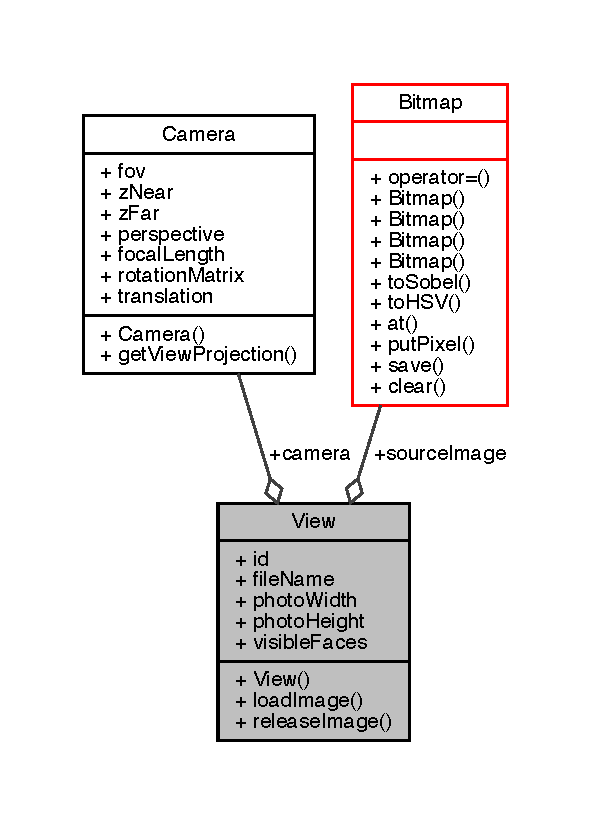
\includegraphics[width=284pt]{class_view__coll__graph}
\end{center}
\end{figure}
\subsection*{Public Member Functions}
\begin{DoxyCompactItemize}
\item 
\hyperlink{class_view_a44ad60a768422d3fa8fbd7576950080a}{View} ()
\item 
void \hyperlink{class_view_a58942806f815fc1f34034c1464aa3d57}{load\+Image} ()
\item 
void \hyperlink{class_view_aa280b349b020b2fb14863b66d054a1da}{release\+Image} ()
\end{DoxyCompactItemize}
\subsection*{Public Attributes}
\begin{DoxyCompactItemize}
\item 
uint \hyperlink{class_view_af416d44fcc5e550f9124cb2227b7c971}{id}
\item 
\hyperlink{class_bitmap}{Bitmap} $\ast$ \hyperlink{class_view_a6694ecbe37c82f827cc5c861ea6544a7}{source\+Image} = nullptr
\item 
std\+::string \hyperlink{class_view_aa525308d25faadf5093d8c368290fb71}{file\+Name}
\item 
\hyperlink{class_camera}{Camera} \hyperlink{class_view_ad7f28c9ee1645c5ba3e1164a29227bf2}{camera}
\item 
uint \hyperlink{class_view_a00c5c1d61a5056a52982e03a6f7f7c70}{photo\+Width}
\item 
uint \hyperlink{class_view_aa6390d1827dd3b222e0a91891c9ff05b}{photo\+Height}
\item 
std\+::unordered\+\_\+set$<$ uint $>$ \hyperlink{class_view_a1c2f222c8f6060c2d3ecb7c08808fa91}{visible\+Faces}
\end{DoxyCompactItemize}


\subsection{Detailed Description}
Class that is used to represent the source image. Hold the information nessecary to recreate and analyse the source image. 

\subsection{Constructor \& Destructor Documentation}
\hypertarget{class_view_a44ad60a768422d3fa8fbd7576950080a}{}\index{View@{View}!View@{View}}
\index{View@{View}!View@{View}}
\subsubsection[{View()}]{\setlength{\rightskip}{0pt plus 5cm}View\+::\+View (
\begin{DoxyParamCaption}
{}
\end{DoxyParamCaption}
)\hspace{0.3cm}{\ttfamily [inline]}}\label{class_view_a44ad60a768422d3fa8fbd7576950080a}


\subsection{Member Function Documentation}
\hypertarget{class_view_a58942806f815fc1f34034c1464aa3d57}{}\index{View@{View}!load\+Image@{load\+Image}}
\index{load\+Image@{load\+Image}!View@{View}}
\subsubsection[{load\+Image()}]{\setlength{\rightskip}{0pt plus 5cm}void View\+::load\+Image (
\begin{DoxyParamCaption}
{}
\end{DoxyParamCaption}
)}\label{class_view_a58942806f815fc1f34034c1464aa3d57}
Loads an image into memory \hypertarget{class_view_aa280b349b020b2fb14863b66d054a1da}{}\index{View@{View}!release\+Image@{release\+Image}}
\index{release\+Image@{release\+Image}!View@{View}}
\subsubsection[{release\+Image()}]{\setlength{\rightskip}{0pt plus 5cm}void View\+::release\+Image (
\begin{DoxyParamCaption}
{}
\end{DoxyParamCaption}
)}\label{class_view_aa280b349b020b2fb14863b66d054a1da}
Releases the image from the memory 

\subsection{Member Data Documentation}
\hypertarget{class_view_ad7f28c9ee1645c5ba3e1164a29227bf2}{}\index{View@{View}!camera@{camera}}
\index{camera@{camera}!View@{View}}
\subsubsection[{camera}]{\setlength{\rightskip}{0pt plus 5cm}{\bf Camera} View\+::camera}\label{class_view_ad7f28c9ee1645c5ba3e1164a29227bf2}
Instance of the camera class that hold camera parameters and position \hypertarget{class_view_aa525308d25faadf5093d8c368290fb71}{}\index{View@{View}!file\+Name@{file\+Name}}
\index{file\+Name@{file\+Name}!View@{View}}
\subsubsection[{file\+Name}]{\setlength{\rightskip}{0pt plus 5cm}std\+::string View\+::file\+Name}\label{class_view_aa525308d25faadf5093d8c368290fb71}
Filename of the source photograph \hypertarget{class_view_af416d44fcc5e550f9124cb2227b7c971}{}\index{View@{View}!id@{id}}
\index{id@{id}!View@{View}}
\subsubsection[{id}]{\setlength{\rightskip}{0pt plus 5cm}uint View\+::id}\label{class_view_af416d44fcc5e550f9124cb2227b7c971}
I\+D that is assigned to a view. Starts at 1 \hypertarget{class_view_aa6390d1827dd3b222e0a91891c9ff05b}{}\index{View@{View}!photo\+Height@{photo\+Height}}
\index{photo\+Height@{photo\+Height}!View@{View}}
\subsubsection[{photo\+Height}]{\setlength{\rightskip}{0pt plus 5cm}uint View\+::photo\+Height}\label{class_view_aa6390d1827dd3b222e0a91891c9ff05b}
Height of the source photo \hypertarget{class_view_a00c5c1d61a5056a52982e03a6f7f7c70}{}\index{View@{View}!photo\+Width@{photo\+Width}}
\index{photo\+Width@{photo\+Width}!View@{View}}
\subsubsection[{photo\+Width}]{\setlength{\rightskip}{0pt plus 5cm}uint View\+::photo\+Width}\label{class_view_a00c5c1d61a5056a52982e03a6f7f7c70}
Widths of the source photo \hypertarget{class_view_a6694ecbe37c82f827cc5c861ea6544a7}{}\index{View@{View}!source\+Image@{source\+Image}}
\index{source\+Image@{source\+Image}!View@{View}}
\subsubsection[{source\+Image}]{\setlength{\rightskip}{0pt plus 5cm}{\bf Bitmap}$\ast$ View\+::source\+Image = nullptr}\label{class_view_a6694ecbe37c82f827cc5c861ea6544a7}
\hyperlink{class_bitmap}{Bitmap} of the source photograph \hypertarget{class_view_a1c2f222c8f6060c2d3ecb7c08808fa91}{}\index{View@{View}!visible\+Faces@{visible\+Faces}}
\index{visible\+Faces@{visible\+Faces}!View@{View}}
\subsubsection[{visible\+Faces}]{\setlength{\rightskip}{0pt plus 5cm}std\+::unordered\+\_\+set$<$uint$>$ View\+::visible\+Faces}\label{class_view_a1c2f222c8f6060c2d3ecb7c08808fa91}
Set of the faces that are visible from the source photo 

The documentation for this class was generated from the following files\+:\begin{DoxyCompactItemize}
\item 
Texture\+Extractor\+V2/\hyperlink{_view_8hpp}{View.\+hpp}\item 
Texture\+Extractor\+V2/\hyperlink{_view_8cpp}{View.\+cpp}\end{DoxyCompactItemize}

%--- End generated contents ---

% Index
\backmatter
\newpage
\phantomsection
\clearemptydoublepage
\addcontentsline{toc}{chapter}{Index}
\printindex

\end{document}
